\chapter{电子能带}\label{sec:electron-band-structure}

本章分析能带电子,所谓能带电子通常是在两个假设下计算出来的:首先是\concept{静态近似},即暂时不考虑晶格振动,只是将晶格当成提供了周期性势场的一个背景;其次是\concept{近独立近似},由于很难一上手就处理带有复杂相互作用的电子气,因此我们首先处理\concept{近独立电子气},也就是电子之间近似没有相互作用的电子气。
近独立假设下单电子哈密顿量为
\begin{equation}
    {H} = \frac{{\vb*{p}}^2}{2m_\text{e}} + V(\vb*{r}),
    \label{eq:single-electron-hamiltonian}
\end{equation}
整团电子气的哈密顿量是关于各个电子的哈密顿量之和。

静态近似需要使用电子-声子相互作用修正。
至于近独立近似,虽然在很多系统中相互作用的影响不能忽略,但能带理论仍然提供了一个很好的“自由理论”,可以在此之上讨论相互作用带来的影响。
例如,\eqref{eq:single-electron-hamiltonian}中的$V(\vb*{r})$可以不是物理意义明确(比如由原子核施加的库伦能)的势能,而有可能是相互作用电子气在一定情况下产生的等效势能。
实际上,对任何一个相互作用系统,都可以找到势$V(\vb*{r})$使得其能量近似可以写成\eqref{eq:single-electron-hamiltonian}的形式(见\eqref{eq:dyson-wave-eq}),但如果相互作用很强,即使往系统中放入一个电子,势$V(\vb*{r})$的形式也会发生很大改变。
此时有时可以使用朗道费米液体理论,保留单电子图像,而将相互作用的影响当成体系总能量的一个修正,但也有可能会得到强关联系统,此时将系统看成近独立电子气并无意义。

\section{周期势场中的自由电子气模型}

\subsection{自由电子气}

现在我们讨论最为简单的近独立电子气,也就是$V(\vb*{r})$在物体内部为常数(可以看成零)的情况。

\subsubsection{能谱和本征态} 

我们在坐标表象下处理问题。计算单个电子的波函数:
\[
    - \frac{\laplacian}{2m_\text{e}} \psi(\vb*{r}) = \epsilon \psi(\vb*{r}),
\]
这种方程的解当然是平面波解的线性组合。一个这样的平面波解形如
\[
    \psi(\vb*{r}) \propto \ee^{\ii \vb*{k} \cdot \vb*{r}}.
\]
只能保证这个式子在物体内部成立,因为物体边界处$V(\vb*{r})$不可能是常数。
然后我们归一化这些平面波。电子可以自发地溢出物体,但是这样的概率并不大,所以我们可以简单地认为电子只会出现在物体内部(也即,物体被放置在一个无限深势陷当中)。设物体体积为$V$,以下我们均使用记号\eqref{eq:integrate-ouver-whole-space},就有
\[
    \int \dd[3]{\vb*{r}} \abs{\psi(\vb*{r})}^2 = 1,
\]
于是
\[
    \psi (\vb*{r}) = \frac{1}{\sqrt{V}} \ee^{\ii \vb*{k} \cdot \vb*{r}}, \quad \epsilon = \frac{k^2}{2m_\text{e}}.
\]
很容易看出这些波函数实际上是动量算符的本征态,$\vb*{k}$实际上就是动量。另一方面,这些波函数定义在坐标空间中,坐标空间中的一切都和自旋算符对易,因此这些波函数也是自旋本征态。于是动量和自旋的一组共同正交本征函数为
\begin{equation}
    \psi_{\vb*{k},\sigma} (\vb*{r}) = \frac{1}{\sqrt{V}} \ee^{\ii \vb*{k} \cdot \vb*{r}}, \quad \epsilon_{\vb*{k},\sigma} = \frac{k^2}{2m_\text{e}}.
\end{equation}
% 真的是这个名字吗?这些波函数称为\concept{Bloch波函数}。
$\vb*{k}$能够取什么值取决于边界条件。由于物体通常比较大,具体取什么样的边界条件对物体内部的过程毫无影响。

\subsubsection{零温状态} 

自由电子气的费米面是球状的(即\concept{费米球})。对三维系统,动量空间中大小为$\dd[3]{\vb*{k}}$的区域内的状态数为
\begin{equation}
    \dd{N} = 2 \frac{V}{(2\pi)^3} \dd[3]{\vb*{k}},
\end{equation}
因子$2$是因为电子有两个自旋。积掉无用的动量分布角自由度就得到
\begin{equation}
    \dd{N} = \frac{V k^2 \dd{k}}{\pi^2}.
\end{equation}
在本问题中,使用“相空间仍然由动量和坐标确定,只不过被划分为相格”的假设也可以推导出正确的$\dd{N}$:我们有
\[
    \dd{N} = 2 \frac{\dd[3]{\vb*{r}} \dd[3]{\vb*{k}}}{(2\pi)^3},
\]
而积掉无用的坐标自由度和动量角自由度之后得到
\[
    \dd{N} = \frac{V k^2 \dd{k}}{\pi^2}.
\]

我们根据能谱计算态密度。由于
\[
    \epsilon = \frac{k^2}{2m},
\]
可以推导出
\[
    \dd{N} = \frac{V (2m)^{3/2} \sqrt{\epsilon} \dd{\epsilon}}{2 \pi^2},
\]
即单位能量间隔中的态有
\begin{equation}
    D(\epsilon) = \frac{V (2m)^{3/2} \sqrt{\epsilon} }{2 \pi^2}
\end{equation}
这么多。这样就可以计算出总粒子数和费米能(即零温化学势)之间的关系:
\begin{equation}
    N = \int_{\epsilon=0}^{\epsilon_{\text{F}}} \dd{N} = \frac{V (2m)^{3/2}}{3 \pi^2} \epsilon_\text{F}^{3/2},
\end{equation}
以及总能量
\begin{equation}
    E = \int_{\epsilon=0}^{\epsilon_{\text{F}}} \epsilon \dd{N} = \frac{V (2m)^{3/2}}{5 \pi^2} \epsilon_\text{F}^{5/2} = \frac{3}{5} N \epsilon_{\text{F}}.
\end{equation}
对二维或者一维的自由电子气也可以使用类似的方法得到系数不同的结论。

\subsubsection{热力学性质} 

我们现在计算有限温下自由电子气的一些热力学性质。
设$Q(\epsilon)$为$\epsilon$下方的所有状态数,即
\begin{equation}
    Q(\epsilon) = \int_0^\epsilon \dd{\epsilon'} D(\epsilon'),
\end{equation}
于是总电子数为
\[
    N = \int_0^\infty \dd{\epsilon} D(\epsilon) f(\epsilon) = \int_0^\infty \dd{\epsilon} Q(\epsilon) \left( - \pdv{f}{\epsilon} \right).
\]
我们有
\[
    - \pdv{f}{\epsilon} = \frac{\beta}{(\ee^{\beta (\epsilon - \mu)} + 1) (\ee^{- \beta (\epsilon - \mu)} + 1)},
\]
它在温度不高时是$\epsilon = \mu$附近的一个尖峰,并且相对于$\epsilon - \mu$是偶函数,从而可以当成一个经过某些修正的$\delta$函数。
这样,我们可以将$N$中的积分下限拓展到$-\infty$而对结果没有太大影响。这样我们有
\[
    \begin{aligned}
        N &= \int_{-\infty}^\infty \dd{\epsilon} Q(\epsilon) \left(-\pdv{f}{\epsilon}\right) \\
        &= \int_{-\infty}^\infty \dd{\epsilon} \left( Q(\mu) + Q'(\mu) (\epsilon - \mu) + \frac{1}{2} Q''(\mu) (\epsilon - \mu)^2 + \cdots \right) \left(-\pdv{f}{\epsilon}\right) .
    \end{aligned}
\]
这其中,第二项一定是零,因为它关于$\epsilon - \mu$是奇函数。
第一项就是
\[
    - \int_{-\infty}^\infty \dd{\epsilon} Q(\mu) \pdv{f}{\epsilon} = Q(\mu) (f(-\infty) - f(\infty)) = Q(\mu), 
\]
而第三项是
\[
    \begin{aligned}
        &\quad \frac{1}{2} Q''(\mu) \int_{-\infty}^\infty \dd{\epsilon} (\epsilon - \mu)^2 \frac{\beta}{(\ee^{\beta (\epsilon - \mu)} + 1) (\ee^{- \beta (\epsilon - \mu)} + 1)} \\
        &= \frac{1}{2 \beta^2} Q''(\mu) \int_{-\infty}^\infty \dd{\xi} \frac{\xi^2}{(\ee^{-\xi} + 1) (\ee^{\xi} + 1)} \\
        &= \frac{\pi^2}{6} Q''(\mu) T^2.
    \end{aligned}
\]
因此在$T^2$精度下我们有
\begin{equation}
    N = Q(\mu) + \frac{\pi^6}{6} Q''(\mu) T^2.
\end{equation}
我们现在尝试写出$\mu$的一个显式表达式。首先$Q(\mu)$和$N$其实是很接近的,可以做展开
\[
    \begin{aligned}
        Q(\mu) - N &= Q(\epsilon_\text{F}) + Q'(\epsilon_\text{F}) (\mu - \epsilon_\text{F}) - N \\
        &= D(\epsilon_\text{F}) (\mu - \epsilon_\text{F}),
    \end{aligned}
\]
因此我们有
\[
    \mu - \epsilon_\text{F} \sim \frac{Q''(\mu)}{D(\epsilon_\text{F})} T^2.
\]
这又意味着展开式
\[
    \frac{\pi^6}{6} Q''(\mu) T^2 = \frac{\pi^6}{6} \left( Q''(\epsilon_\text{F}) + Q'''(\epsilon_\text{F}) (\epsilon_\text{F} - \mu) + \cdots \right) T^2
\]
中的第一项就达到了$T^2$的精度,从而如果我们只需要计算到$T^2$精度,只需要求解
\[
    D(\epsilon_\text{F}) (\mu - \epsilon_\text{F}) + \frac{\pi^2}{6} Q''(\epsilon_\text{F}) T^2 = 0
\]
即可,最终计算得到
\begin{equation}
    \mu = \epsilon_\text{F} \left( 1 - \frac{\pi^2}{12} \left( \frac{T}{\epsilon_\text{F}} \right)^2 + \cdots \right).
\end{equation}

类似地计算热容,电子贡献的内能为
\[
    U = \int_0^\infty \dd{\epsilon} \epsilon f(\epsilon) D(\epsilon),
\]
类似地引入
\[
    R(\epsilon) = \int_0^\infty \dd{\epsilon} \epsilon D(\epsilon),
\]
做分部积分,泰勒展开,
\begin{equation}
    C_V = \frac{n \pi^2}{2} \frac{T}{T_\text{F}},
    \label{eq:free-electron-special-heat}
\end{equation}
与经典Drude模型非常不一样。直观地看,这是因为只有费米面附近的电子才会被激发。

\subsection{周期势}\label{sec:periodic-potential-electron}

在Bloch定理中我们没有看到周期势场具体是怎样让能带产生的,以及能带编号$n$到底标记了哪些自由度。
下面我们将自由电子放在周期势场中做微扰计算,来更清楚地看到能带如何形成。
本节开始给出自由电子放在周期势场中而形成能带这一事实的具体计算。

设周期势场为$V(\vb*{r})$,它导致的一阶能量修正为
\begin{equation}
    \epsilon_{\vb*{k}}^{(1)} = \mel{\vb*{k}}{V}{\vb*{k}} = \bar{V},
\end{equation}
就是周期势的空间平均。因此如下我们将$\bar{V}$归入$\epsilon_{\vb*{k}}^{(0)}$中,或者也可以归入化学势中,而认为周期势场的空间平均是零。
二阶非简并微扰论给出
\begin{equation}
    \epsilon_{\vb*{k}}^{(2)} = \sum_{\vb*{k} \neq \vb*{k}'} \frac{\abs{\mel*{\vb*{k}'}{V}{\vb*{k}}}^2}{\epsilon_{\vb*{k}}^{(0)} - \epsilon_{\vb*{k}'}^{(0)}},
\end{equation}
由于周期性,有(我们其实是在使用\eqref{eq:sqrt-v-rep},但是由于是在展开算符,归一化常数为$(1/\sqrt{V})^2 = 1 / V$)
\begin{equation}
    \begin{aligned}
        \mel*{\vb*{k}'}{V}{\vb*{k}} &= \frac{1}{V} \int \dd[3]{\vb*{r}} V(\vb*{r}) \ee^{\ii (\vb*{k} - \vb*{k}') \cdot \vb*{r}} \\
        &= \frac{1}{V_\text{u.c.}} \int_\text{u.c.} \dd[3]{\vb*{r}} V(\vb*{r}) \ee^{\ii (\vb*{k} - \vb*{k}') \cdot \vb*{r}} \frac{1}{N} \sum_m \ee^{\ii (\vb*{k} - \vb*{k}') \cdot \vb*{R}_i} \\
        &= \frac{1}{V_\text{u.c.}} \sum_n \delta_{\vb*{k} - \vb*{k}' + \vb*{G}_n} \int_\text{u.c.} \dd[3]{\vb*{r}} V(\vb*{r}) \ee^{- \ii \vb*{G}_n \cdot \vb*{r}} \eqqcolon \sum_n \delta_{\vb*{k} - \vb*{k}' + \vb*{G}_n} V_n,
    \end{aligned}
\end{equation}
这里我们定义了
\begin{equation}
    V_n = \frac{1}{V_\text{u.c.}} \int_\text{u.c.} \dd[3]{\vb*{r}} V(\vb*{r}) \ee^{- \ii \vb*{G}_n \cdot \vb*{r}}.
\end{equation}
于是计算得到
\begin{equation}
    \epsilon_{\vb*{k}}^{(2)} = \sum_{n} \delta_{\vb*{k} - \vb*{k}' + \vb*{G}_n} \frac{\abs{V_n}^2}{\epsilon_{\vb*{k}}^{(0)} - \epsilon_{\vb*{k}'}^{(0)}} .
\end{equation}
因此,只要非简并微扰论适用,周期势场做的就是修正一下单电子能级。
修正了的波函数为
\begin{equation}
    \psi_{\vb*{k}}^{(1)} = \sum_{\vb*{G}_n} \ee^{\ii (\vb*{k} + \vb*{G}_n) \cdot \vb*{r}} \frac{V_n}{\epsilon_{\vb*{k}}^{(0)} - \epsilon_{\vb*{k} + \vb*{G}_n}^{(0)}}.
    .
    \label{eq:non-degenerate-wave-function} 
\end{equation}

然而,在
\begin{equation}
    \abs{\vb*{k}}^2 = \abs*{\vb*{k} + \vb*{G}_n}^2
    \label{eq:brillouin-condition}
\end{equation}
时,非简并微扰论发散。此时应当使用简并微扰。由于满足这一条件的$\vb*{k}$和$\vb*{k} + \vb*{G}_n$在三维情况下很多,我们此处不做一般的计算。
\eqref{eq:brillouin-condition}的几何意义是$\vb*{k}$在起点位于原点的$-\vb*{G}_n$的垂直平分面上。
回顾布里渊区的概念,我们发现此时$\vb*{k}$一定在某两个布里渊区的交界面上。
我们现在将每个电子模式的$\vb*{k}$适当地加上或者减去一个倒格矢,将动量在第一布里渊区以外的所有模式都移动到第一布里渊区以内,即于将单电子能谱平移任意一个倒格矢,然后将第一布里渊区以外的部分全部抹除掉,则彼此之间存在能量简并,并且只相差一个倒格矢的电子模式具有非常直观的特点:它们是第一布里渊区边界上的简并。
现在加上周期势,在第一布里渊区内部,能级只是发生小的修正,在边界处,简并微扰导致交叉点“退开”,自我交叉的单一能带分离成一系列不相交的波浪线,这就得到了一系列不同的能带。
此时我们说,能带之间\concept{打开了能隙}或者说\concept{回避交叉},让原本交叉的能带之间出现了间隙。

因此,布里渊区的概念在能带论中是一定会出现的:只有在布里渊区边界上,会出现必须使用简并微扰论、在自由电子情况下简并的能级打开能隙(从而连续的能谱断开)等现象。
在远离布里渊区边界的地方,周期势场只会修正能级能量,不会改变能带的连续性。
我们通过一个具体例子看到了为什么通常将第一布里渊区作为倒空间原胞。

以上使用的$\vb*{k}$都对应着某个平面波的真正的波矢(我们称它为\concept{广延波矢},和约束在某个倒空间原胞中的晶格波矢相区分)。
在周期势场下第一布里渊区边界上简并解除,原本连续的自由电子能谱分离成若干条能带,从而我们可以使用能带编号$n$和通过加减特定倒格矢回到第一布里渊区中的$\vb*{k}$标记各个电子模式。
\concept{晶格动量}就是把自由电子的广延动量加减特定倒格矢挪到第一布里渊区中,因此也可以称为\concept{简约动量}。
波函数的微扰论(非简并微扰有\eqref{eq:non-degenerate-wave-function},简并微扰发生在彼此差一个倒格矢的模式之间)显示一个Bloch波函数的简约动量和构成它的各个自由电子波函数分量的广延动量之间只差一个倒格矢,因此,在相差一个倒格矢的意义上,可以认为电子的简约动量和广延动量是一回事。
同时,无论是非简并微扰的微扰后波函数\eqref{eq:non-degenerate-wave-function}还是简并微扰的微扰后波函数都满足
\[
    \psi(\vb*{r} + \vb*{R}_i) = \ee^{\ii \vb*{k} \cdot \vb*{R}_i} \psi(\vb*{r}),
\]
因此简约波矢$\vb*{k}$实际上就是Bloch定理中的那个$\vb*{k}$,即晶格动量。

\begin{figure}
    \centering
    \subfigure[自由空间中的单电子能谱]{
        \begin{tikzpicture}
        
            % 动量横轴
            \draw[->] (-3,0) -- (3,0) node[right] {$\vb*{k}$};
            % 动能纵轴
            \draw[->] (0,-0.25) -- (0,6) node[above] {$\epsilon_{\vb*{k}}$};
            
            % 画出$\epsilon_{\vb*{k}}$曲线
            \draw[samples=50, smooth, domain=-3:3] plot(\x,{0.5*(\x*\x)});
    
        \end{tikzpicture}
    }
    \subfigure[由于晶格的周期性,出现第一布里渊区折叠,能谱在第一布里渊区外的部分移动回到第一布里渊区中,在简并微扰中彼此会有影响的态体现为第一布里渊区边界上的简并]{
        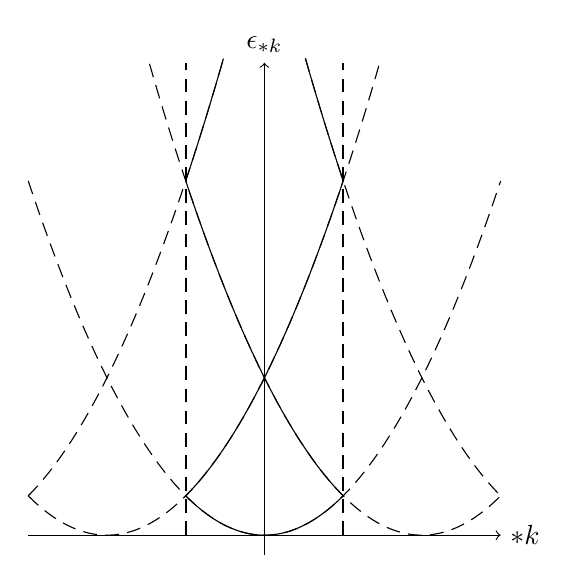
\begin{tikzpicture}
        
            % 动量横轴
            \draw[->] (-3,0) -- (3,0) node[right] {$\vb*{k}$};
            % 动能纵轴
            \draw[->] (0,-0.25) -- (0,6) node[above] {$\epsilon_{\vb*{k}}$};

            % 布里渊区边界
            \draw[dash pattern=on5pt off3pt, thick] (-1, 0) -- (-1, 6);
            \draw[dash pattern=on5pt off3pt, thick] (1, 0) -- (1, 6);
            
            % 画出布里渊区以外的能谱
            
            \draw[dash pattern=on5pt off3pt,samples=50, smooth, domain=-3:1.46] plot(\x,{0.5*((\x+2)*(\x+2))});
            \draw[dash pattern=on5pt off3pt,samples=50, smooth, domain=-3:3] plot(\x,{0.5*((\x)*(\x))});
            \draw[dash pattern=on5pt off3pt,samples=50, smooth, domain=-1.46:3] plot(\x,{0.5*((\x-2)*(\x-2))});
            \draw[dash pattern=on5pt off3pt,samples=50, smooth, domain=0.52:3] plot(\x,{0.5*((\x-4)*(\x-4))});
            \draw[dash pattern=on5pt off3pt,samples=50, smooth, domain=-3:-0.52] plot(\x,{0.5*((\x+4)*(\x+4))});

            % 画出布里渊区内部的$\epsilon_{\vb*{k}}$曲线,以及由于晶格周期性而导致的能谱平移
            \draw[samples=50, smooth, domain=-1:1] plot(\x,{0.5*(\x*\x)});
            \draw[samples=50, smooth, domain=-1:1] plot(\x,{0.5*((\x-2)*(\x-2))});
            \draw[samples=50, smooth, domain=-1:1] plot(\x,{0.5*((\x+2)*(\x+2))});
            \draw[samples=50, smooth, domain=0.52:1] plot(\x,{0.5*((\x-4)*(\x-4))});
            \draw[samples=50, smooth, domain=-1:-0.52] plot(\x,{0.5*((\x+4)*(\x+4))});
    
        \end{tikzpicture}
        
    }
    \subfigure[相互作用打开能隙,形成分离的能带]{
        \tikzset{every picture/.style={line width=0.75pt}} %set default line width to 0.75pt        

        \begin{tikzpicture}[x=0.75pt,y=0.75pt,yscale=-1,xscale=1]
        %uncomment if require: \path (0,419); %set diagram left start at 0, and has height of 419
        
        %Straight Lines [id:da08007999422317735] 
        \draw    (241,378.33) -- (424,378.33) -- (492,378.33) ;
        \draw [shift={(494,378.33)}, rotate = 180] [fill={rgb, 255:red, 0; green, 0; blue, 0 }  ][line width=0.08]  [draw opacity=0] (12,-3) -- (0,0) -- (12,3) -- cycle    ;
        %Straight Lines [id:da14542076195177844] 
        \draw    (370,392) -- (370,48.33) ;
        \draw [shift={(370,46.33)}, rotate = 450] [fill={rgb, 255:red, 0; green, 0; blue, 0 }  ][line width=0.08]  [draw opacity=0] (12,-3) -- (0,0) -- (12,3) -- cycle    ;
        %Straight Lines [id:da21706633188496327] 
        \draw  [dash pattern={on 4.5pt off 4.5pt}]  (311,53.33) -- (311,378.33) ;
        %Straight Lines [id:da010943491501953284] 
        \draw  [dash pattern={on 4.5pt off 4.5pt}]  (430,53.33) -- (430,378.33) ;
        %Curve Lines [id:da7601767287685084] 
        \draw    (311,348) .. controls (334,347.67) and (354,379) .. (370,378.33) ;
        %Curve Lines [id:da7714867177526292] 
        \draw    (429,348) .. controls (406,347.67) and (386,379) .. (370,378.33) ;
        %Curve Lines [id:da295042466286602] 
        \draw    (311,329) .. controls (345,328) and (358,249) .. (370,249) ;
        %Curve Lines [id:da04705148565499395] 
        \draw    (429,329) .. controls (395,328) and (382,249) .. (370,249) ;
        %Curve Lines [id:da3411641649050148] 
        \draw    (311,152) .. controls (345,153) and (361,235) .. (370,237) ;
        %Curve Lines [id:da029058562157771473] 
        \draw    (429,152) .. controls (395,153) and (378,237) .. (370,237) ;
        %Curve Lines [id:da258083133455941] 
        \draw    (311,130) .. controls (330,131) and (336,91) .. (346,49) ;
        %Curve Lines [id:da5337325730240392] 
        \draw    (430,130) .. controls (411,131) and (405,91) .. (395,49) ;

        % Text Node
        \draw (496,378.33) node [anchor=west] [inner sep=0.75pt]    {$\boldsymbol{k}$};
        % Text Node
        \draw (369,42.33) node [anchor=south] [inner sep=0.75pt]    {$\epsilon _{\boldsymbol{k}}$};
                
        % \draw   (370, 378.33) circle [x radius= 5, y radius= 5]   ;
        \end{tikzpicture}

        
    }
    \caption{能带结构}
    \label{fig:bloch-energy-band}
\end{figure}

\subsection{赝势}\label{sec:pseudopotential}

前述的周期势场$V(\vb*{r})$的来源没有明确指出。如果我们将它取为原子核提供的库伦势场,能量最低的那些能带对应的电子状态通常都是非常局域化的原子内层电子,它们的行为和没有形成晶体时的原子的内层电子应该不会有太大区别。
这些电子和原子核就形成了所谓离子实。电子是费米子,因此外层电子不会占据这些轨道,这就产生了一个等效的排斥力。
实际上,这个等效的排斥反而能够简化计算,因为这意味着外层电子感受不到原子核的势场最为奇异的那部分,从而外层电子波函数在接近原子核的区域的高频振荡可以忽略,从而使用几个平面波就能够足够精确地描写它,微扰论总是适用,等等。
这个等效的排斥力是泡利不相容原理的一个例子——即使不考虑电子-电子库伦排斥,内层电子的存在本身就能够导致一个等效排斥力。

本节给出一种比较系统的考虑内层电子轨道对外层电子的影响,但是又不需要真的计算内层电子轨道的作用(或者说不需要做\concept{全电子计算})的方法。
离子实中的核心电子轨道和价电子轨道同时都是单电子哈密顿量的本征态:
\begin{equation}
    H \ket{\psi_c} = E_c \ket{\psi_c}, \quad H \ket{\psi_\text{v}} = E_\text{v} \ket{\psi_\text{v}},
\end{equation}
这里$c$标记了各个内层电子轨道。定义
\begin{equation}
    \ket{\psi_\text{v}^\text{PS}} = \ket{\psi_\text{v}} + \sum_c \ket{\psi_c} \braket*{\psi_c}{\psi_\text{v}^\text{PS}},
\end{equation}
则计算得到
\[
    (H - E_\text{v}) \ket{\psi_\text{v}^\text{PS}} = \sum_c (E_c - E_\text{v}) \ket{\psi_c} \braket*{\psi_c}{\psi_\text{v}^\text{PS}},
\]
从而
\begin{equation}
    \left(H - \sum_c (E_c - E_\text{v}) \dyad*{\psi_c}\right) \ket{\psi_\text{v}^\text{PS}} = E_\text{v} \ket{\psi_\text{v}^\text{PS}}.
    \label{eq:original-pseudopotential}
\end{equation}
这意味着可以定义一个等效的“势”
\begin{equation}
    V^\text{PS} = V - \sum_c (E_c - E_\text{v}) \dyad*{\psi_c},
\end{equation}
从这个势出发做计算能够得到正确的能谱,而价电子波函数则和实际情况不同。
在$\vb*{r}$比较大的地方,$\psi_c(\vb*{r})$很小,从而$V^\text{PS}$和$V$没有差别,在相应的位置上$\psi_\text{v}^\text{PS}(\vb*{r})$和$\psi_\text{v}(\vb*{r})$也没有区别。

到这里我们都没有做任何近似。内层电子的行为的复杂性体现在$V^\text{PS}$显含$E_\text{v}$这件事上。
然而,$E_\text{v}$完全由$\ket{\psi_\text{v}}$的标签确定,而通常单单依靠对称性分析我们就能够知道这些标签是什么。
因此看起来似乎不像本征值问题的\eqref{eq:original-pseudopotential}实际上真的就是一个本征值问题
\begin{equation}
    \left( \frac{\vb*{p}^2}{2m} + V^\text{PS} \right) \ket{\psi_\text{v}^\text{PS}} = E_\text{v} \ket{\psi_\text{v}^\text{PS}}.
\end{equation}
然而,和通常的定态薛定谔方程不同,以上方程中$V^\text{PS}$是依赖于$\ket{\psi_\text{v}^\text{PS}}$的诸如晶格动量(在计算能带时)或是$l$(在求解单原子问题时)的标签的。
实际上这也意味着$V^\text{PS}$在坐标表象下的矩阵元一般来说是$V(\vb*{r}, \vb*{r}')$,而不是局域的$V(\vb*{r})$。

先做单原子的全电子计算,得到电子能级$E^\text{AE}$和波函数$\psi^\text{AE}(\vb*{r})$,然后将单电子轨道波函数$\psi^\text{AE}(\vb*{r})$对球谐函数基底展开,做截断,即只取前几个球谐波,得到$\psi^\text{PS}(\vb*{r})$,然后拟合出一个$V^\text{PS}$使得
\begin{equation}
    - \frac{\laplacian}{2m} \psi^\text{PS}(\vb*{r}) + V^\text{PS}(\vb*{r}) \psi^\text{PS}(\vb*{r}) = E^\text{AE} \psi^\text{PS}(\vb*{r}),
\end{equation}
就得到了一个赝势。在远离原子核的地方$l$较低的球谐函数占据主导地位,因此在那里$\psi^\text{PS}$和$\psi^\text{AE}$是一样的,从而$V^\text{PS}$和$V^\text{AE}$是一样的。
在接近原子核的地方显然$\psi$
相应的,$V^\text{PS}$相较于实际的$V^\text{AE}$要平滑得多。

由于远离原子核时势场快速下降(我们现在尚未考虑电子-电子库伦排斥,电子-电子库伦排斥会屏蔽原子核的势场),在晶体中,非常接近一个原子核处的波函数的形式对另一个原子的势场导致的能级修正而言是不重要的。
因此可以预期,只要赝势和实际的势场相符合的区域稍微大一些,用赝势做能带计算就能够得到正确的结果。

\subsection{$\vb*{k} \cdot \vb*{p}$模型和有效质量}

设我们需要计算$\vb*{k}_0$附近电子的行为。定义
\begin{equation}
    \chi_{n \vb*{k}}(\vb*{r}) = \ee^{\ii (\vb*{k} - \vb*{k}_0) \cdot \vb*{r}} \psi_{n \vb*{k}_0} = \ee^{\ii \vb*{k} \cdot \vb*{r}} u_{n \vb*{k}_0} (\vb*{r}),
\end{equation}
我们来验证正交性和完备性均成立。首先
\[
    \begin{aligned}
        \int \dd[3]{\vb*{r}} \chi^*_{n \vb*{k}}(\vb*{r}) \chi_{m \vb*{k}'}(\vb*{r}) &= \sum_{i} \int_\text{u.c.} \dd[3]{\vb*{r}} \ee^{\ii (\vb*{k}' - \vb*{k}) \cdot (\vb*{r} + \vb*{R}_i)} u^*_{n \vb*{k}_0}(\vb*{r}) u_{m \vb*{k}_0}(\vb*{r}) \\
        &= N \delta_{\vb*{k} \vb*{k}'} \int_\text{u.c.} \dd[3]{\vb*{r}} \ee^{\ii (\vb*{k}' - \vb*{k}) \cdot \vb*{r}} u^*_{n \vb*{k}_0}(\vb*{r}) u_{m \vb*{k}_0}(\vb*{r}) \\
        &= N \delta_{\vb*{k} \vb*{k}'} \int_\text{u.c.} \dd[3]{\vb*{r}} u^*_{n \vb*{k}_0}(\vb*{r}) u_{m \vb*{k}_0}(\vb*{r}) \\
        &= \delta_{\vb*{k} \vb*{k}'} \delta_{mn},
    \end{aligned}
\]
即正交性成立。另一方面通过数自由度也可以发现完备性应该成立。
因此,$\chi_{n \vb*{k}}$构成晶体中电子的一组正交完备基底。

于是我们可以以$\chi_{n \vb*{k}}$为基底尝试对角化哈密顿量。
我们有
\[
    \begin{aligned}
        H \psi_{n \vb*{k}} &= \sum_j \braket*{\chi_{j \vb*{k}}}{\psi_{n \vb*{k}}} \left( \frac{\vb*{p}^2}{2m} + V \right) \chi_{j \vb*{k}} \\
        &= \sum_j \braket*{\chi_{j \vb*{k}}}{\psi_{n \vb*{k}}} \left( \frac{\vb*{p}^2}{2m} + V \right) \ee^{\ii (\vb*{k} - \vb*{k}_0) \cdot \vb*{r}} \psi_{j \vb*{k}_0} \\
        &= \sum_j \braket*{\chi_{j \vb*{k}}}{\psi_{n \vb*{k}}} \ee^{\ii (\vb*{k} - \vb*{k}_0) \cdot \vb*{r}} \left( \frac{(\vb*{p} + \vb*{k} - \vb*{k}_0)^2}{2m} + V \right) \psi_{j \vb*{k}_0} \\
        &= \ee^{\ii (\vb*{k} - \vb*{k}_0) \cdot \vb*{r}} \sum_j \braket*{\chi_{j \vb*{k}}}{\psi_{n \vb*{k}}} \left( \frac{\vb*{p}^2}{2m} + V + \frac{(\vb*{k} - \vb*{k}_0) \cdot \vb*{p}}{m} + \frac{(\vb*{k} - \vb*{k}_0)^2}{2m} \right) \psi_{j \vb*{k}_0} \\
        &= \ee^{\ii (\vb*{k} - \vb*{k}_0) \cdot \vb*{r}} \sum_j \braket*{\chi_{j \vb*{k}}}{\psi_{n \vb*{k}}} \left( \epsilon_{j \vb*{k}_0} + \frac{(\vb*{k} - \vb*{k}_0) \cdot \vb*{p}}{m} + \frac{(\vb*{k} - \vb*{k}_0)^2}{2m} \right) \psi_{j \vb*{k}_0},
    \end{aligned}
\]
而另一方面
\[
    H \psi_{n \vb*{k}} = \epsilon_{n \vb*{k}} \psi_{n \vb*{k}} = \epsilon_{n \vb*{k}} \sum_j \braket*{\chi_{j \vb*{k}}}{\psi_{n \vb*{k}}} \chi_{j \vb*{k}} =  \epsilon_{n \vb*{k}} \sum_j \braket*{\chi_{j \vb*{k}}}{\psi_{n \vb*{k}}} \ee^{\ii (\vb*{k} - \vb*{k}_0) \cdot \vb*{r}} \psi_{n \vb*{k}_0},
\]
于是
\begin{equation}
    \sum_j \braket*{\chi_{j \vb*{k}}}{\psi_{n \vb*{k}}} \left( \left( \epsilon_{n \vb*{k}_0} - \epsilon_{n \vb*{k}} + \frac{(\vb*{k} - \vb*{k}_0)^2}{2m} \right) \delta_{nj} + \frac{(\vb*{k} - \vb*{k}_0) \cdot \mel{\psi_{n \vb*{k}_0}}{\vb*{p}}{\psi_{j \vb*{k}_0}}}{m} \right)  = 0.
    \label{eq:k-p-model}
\end{equation}
我们还可以将以上所有推导中的$\psi_{n \vb*{k}_0}$换成$u_{n \vb*{k}_0}$,此时$\vb*{k} - \vb*{k}_0$被$\vb*{k}$取代,我们有

既然我们已经知道了$\vb*{k}_0$点的电子的情况——它的能级,波函数等等——上式中的仅有的未知数就是$\braket*{\chi_{j \vb*{k}}}{\psi_{n \vb*{k}}}$和$\epsilon_{n \vb*{k}}$,于是可以通过求解本征值问题得到它们。
这就是所谓的\concept{$\vb*{k} \cdot \vb*{p}$理论}。

原则上以上做法能够给出所有能带信息,但是,\eqref{eq:k-p-model}可以很容易地近似求解。
例如,

\begin{equation}
    \left(\frac{1}{m^*}\right)_{\alpha \beta} = \pdv[2]{\epsilon_{\vb*{k}}}{k_\alpha}{k_\beta},
    \label{eq:effective-mass}
\end{equation}
我们将在\autoref{sec:bloch-wave-pocket}中看到有效质量的应用。

能带越宽,有效质量越轻,能带越窄,有效质量越重。\concept{重费米子系统}指的是有效质量非常大的系统,从而这样的系统基本上是强关联系统。

Luttinger模型:能带反转?

\section{Bloch波函数和Wannier波函数}

本节给出周期性势场中的近独立电子气的一些一般性质。

\subsection{Bloch定理}\label{sec:bloch-electron}

\autoref{sec:transition-group-rep}中的Bloch定理当然适用于近独立电子气模型,因此这种模型中的电子的波函数自然服从\eqref{eq:bloch-wavefunction}。我们在处于这种状态的电子称为\concept{Bloch电子}。
能带电子总是可以认为是自由电子加入了足够多的微扰之后得到的,而我们在\autoref{sec:periodic-potential-electron}最后提到过,\eqref{eq:bloch-wavefunction}中的那个晶格动量$\vb*{k}$和组成Bloch电子的诸多平面波分量的波矢(即自由电子的真正的动量,或者说延展动量)最多差一个倒格矢。
因此,晶格动量为$\vb*{k}$的Bloch电子可以认为是携带了真实的动量,这动量是$\vb*{k}$,$\vb*{k}+\vb*{G}_i$,$\vb*{k} + \vb*{G}_j$等一系列延展动量的混合,而自由电子做了足够多的微扰之后得到的波函数其实就是这种系统的Bloch波函数。

我们现在来看$n$代表什么。Bloch电子显然满足一个周期性边界条件,因此它是某个等效单电子哈密顿量的周期性解。
将\eqref{eq:bloch-wavefunction}代入
\[
    -\frac{\laplacian}{2m_\text{e}} \psi(\vb*{r}) + V(\vb*{r}) \psi(\vb*{r}) = \epsilon \psi(\vb*{r}),
\]
得到
\begin{equation}
    \left( - \frac{(\grad+ \ii \vb*{k})^2}{2m_\text{e}} + V(\vb*{r}) \right) u_{\vb*{k}}(\vb*{r}) = \epsilon u_{\vb*{k}}(\vb*{r}).
    \label{eq:block-energy-problem}
\end{equation}
在$\vb*{k}$已知的情况下求解该本征值问题,可以得到一组$u$以及对应的$E$。由于先前要求$u(\vb*{r})$是周期函数,该本征值问题必定给出离散谱,也即,我们会获得一组$(\psi_{n \vb*{k}}, \epsilon_{n \vb*{k}})$,使得
\begin{equation}
    \left( - \frac{(\grad+\ii \vb*{k})^2}{2m_\text{e}} + V(\vb*{r}) \right) u_{n \vb*{k}}(\vb*{r}) = \epsilon_{n \vb*{k}} u_{n \vb*{k}}(\vb*{r}),
    \label{eq:eigen-function-bloch-u}
\end{equation}
$n$是另一个(离散的)好量子数,我们现在看到它是单个晶胞中的离散谱的能级标记。

通过数自由度我们还可以看出$n$的另一个意义:$\vb*{k}$对应着晶格,从而$n$对应着一个晶胞中不同的原子以及每个原子周围的电子轨道。
当然,原则上原子周围有无数个电子轨道,从而$n$可以任意的大,但是实际上我们通常会在某一个能量尺度上截断,物理上,这是因为特别高的空轨道对低能过程没有什么影响。
一旦$\vb*{k}$和$n$给定,Bloch波函数及其时间演化就完全求解出来了,从而$\vb*{k}$和$n$是坐标空间中的Bloch波函数的全部好量子数。我们称取不同$n$值的电子处于不同的\concept{能带}上,$n$为能带标记。%
\footnote{注意到,能带的导出实际上并未用到太多晶体的性质(空间周期性等),因此非晶体很多时候也有能带。}%
能带中的电子在空间上非常不定域,它们实际上是一系列格点上的定域态叠加而成的结果。也可以这么理解这一点:写出一个格点上的哈密顿量之后为了计算能带能量肯定要做对角化,对角化得到的本征向量肯定是把一系列格点上的定域态都线性组合起来了。
总之,能带中的Bloch电子常常称为\concept{巡游电子}。

由于晶体近似在一个无限深势阱中,波函数在晶体边界处快速衰减为零。这就意味着$\vb*{k}$实际上是离散的。然而,由于晶体的尺度通常远大于原子的尺度,$\vb*{k}$近似可认为是连续的。于是可以写出函数
\[
    \epsilon = \epsilon_n(\vb*{k}),
\]
由于$\vb*{k}$加上任何一个倒格矢之后给出同样的Bloch波函数,$E$相对于$\vb*{k}$应该具有周期性,那么它必定是有界的。
这就是“能带”这个名称的来源:穷举一个倒空间原胞内部的所有$\vb*{k}$,得到的所有能量组成一条有限宽的条带。

两条不同的能带之间的间隙提供了一个自然的能量截断,因此在我们已经知道了系统的能带之后,如果需要一个低能有效理论,可以只考虑能量较低的能带,而将粒子跃迁到能量较高的能带再跃迁回来作为微扰,进行能量修正,即可以很自然地将高能能带积掉。

最后我们指定波函数的归一化方式。我们这里做的内积操作是\autoref{sec:momentum-space-inner-product}中的第一种情况,即对全空间积分。
可以使用约定\eqref{eq:integrate-ouver-whole-space}。
此时由
\begin{equation}
    \int \dd[3]{\vb*{r}} \psi_{n \vb*{k}}^*(\vb*{r}) \psi_{m \vb*{k}'}(\vb*{r}) = \delta_{mn} \delta_{\vb*{k} \vb*{k}'}
\end{equation}
可以得出
\[
    \begin{aligned}
        \delta_{mn} \delta_{\vb*{k} \vb*{k}'} &= \sum_{i} \int_\text{u.c.} \dd[3]{\vb*{r}} \ee^{- \ii (\vb*{R}_i + \vb*{r}) \cdot \vb*{k}} u_{n \vb*{k}}^*(\vb*{r}) \ee^{\ii (\vb*{R}_i + \vb*{r}) \cdot \vb*{k}'} u_{m \vb*{k}'}(\vb*{r}) \\
        &= N \delta_{\vb*{k} \vb*{k}'} \int_\text{u.c.} \dd[3]{\vb*{r}} \ee^{- \ii (\vb*{k} - \vb*{k}') \cdot \vb*{r}} u_{n \vb*{k}}^*(\vb*{r}) u_{m \vb*{k}'}(\vb*{r}) \\
        &= N \delta_{\vb*{k} \vb*{k}'} \int_\text{u.c.} \dd[3]{\vb*{r}} u_{n \vb*{k}}^*(\vb*{r}) u_{m \vb*{k}'}(\vb*{r}),
    \end{aligned}
\]
于是
\[
    \int_\text{u.c.} \dd[3]{\vb*{r}} u^*_{n \vb*{k}}(\vb*{r}) u_{m \vb*{k}}(\vb*{r}) = \frac{1}{N},
\]
或者考虑$u_{n \vb*{k}}$的周期性,有
\begin{equation}
    \int \dd[3]{\vb*{r}} u^*_{n \vb*{k}}(\vb*{r}) u_{m \vb*{k}}(\vb*{r}) = \delta_{mn}. 
\end{equation}

如果使用\eqref{eq:integrate-ouver-whole-space-divided},则
\begin{equation}
    \frac{1}{V} \int \dd[3]{\vb*{r}} \psi_{n\vb*{k}}^*(\vb*{r}) \psi_{m\vb*{k}'}(\vb*{r}) = \delta_{mn} \delta_{\vb*{k} - \vb*{k}'},
    \label{eq:bloch-is-basis}
\end{equation}
从而让简单的平面波$\exp(\ii \vb*{k} \cdot \vb*{r})$不需要乘上归一化因子就能够成为归一化本征态。
设$V_\text{u.c.}$是单个晶胞的大小,则
\[
    V = N V_\text{u.c.},
\]
从而可以得到
\begin{equation}
    \frac{1}{V_\text{u.c.}} \int_\text{u.c.} \dd[3]{\vb*{r}} u_{m\vb*{k}}^*(\vb*{r}) u_{n\vb*{k}}(\vb*{r}) = \delta_{mn}.
\end{equation}
只需要求解出一组满足以上条件的$\{u_{n\vb*{k}}\}$,就得到了一组正交归一化波函数$\{\psi_{n\vb*{k}}\}$。
归一化系数使用$V_\text{u.c.}$是非常合理的,因为如\eqref{eq:normalization-periodic}所示这正是具有正格子的周期性的函数通常使用的归一化系数,这里$u_{n \vb*{k}}$的地位和$\ee^{\ii \vb*{k} \cdot \vb*{r}}$相同。

\eqref{eq:bloch-is-basis}意味着Bloch波函数是正交归一化波函数且对应的积分测度为
\[
    \frac{1}{\sqrt{V}} \int \dd[3]{\vb*{r}},
\]
记${c}_{n\vb*{k}}^\dagger$为位于能带$n$、晶格动量为$\vb*{k}$的Bloch电子的产生算符,那么%
\footnote{其中的$1/\sqrt{V}$的因子是因为二次量子化场算符通常使用全空间的积分为内积的定义,在此定义下,归一化的波函数是$\psi_{n\vb*{k}} / \sqrt{V}$而不是$\psi_{n\vb*{k}}$。
换句话说,在归一化\emph{波函数}$\psi_{n \vb*{k}}$时我们使用了约定\eqref{eq:v-rep},而归一化\emph{场算符}时我们使用了约定\eqref{eq:sqrt-v-rep}。
}%
\begin{equation}
    {c}_{n \vb*{k}}^\dagger = \frac{1}{\sqrt{V}} \int \dd[3]{\vb*{r}} \psi_{n \vb*{k}}(\vb*{r}) {\psi}^\dagger(\vb*{r}), \quad \psi^\dagger(\vb*{r}) = \frac{1}{\sqrt{V}} \sum_{\vb*{k}} \psi_{n \vb*{k}}(\vb*{r})^* c_{n \vb*{k}}.
    \label{eq:bloch-transformation}
\end{equation}
这和\eqref{eq:sqrt-v-rep}非常类似,不同之处在于此时的积分变换核中多了一个周期性的$u_{n \vb*{k}}$,并且除了$\vb*{k}$以外还有离散的标签$n$。
哈密顿量在这一组基下是对角化的,于是写出二次量子化哈密顿量(已经加入化学势项)
\begin{equation}
    {H} = \sum_{n, \vb*{k}} (\epsilon_{n\vb*{k}} - \mu) {c}^\dagger_{n\vb*{k}} {c}_{n\vb*{k}}.
    \label{eq:bloch-band-hamiltonian}
\end{equation}
$\vb*{k}$的取值局限在第一布里渊区内部,作为对比,不考虑周期势的边长为$L$的正方体势阱中的电子的$\vb*{k}$可以取遍所有位于那个边长为$2\pi / L$的格点。
但实际上两者的自由度是一样的,因为我们还有$n$标记各个能带,也即,我们相当于把所有能带中的动量都移动到了第一布里渊区内部。

以上讨论并没有说明我们应该将$\vb*{k}$约束在\emph{哪一个}倒格子原胞中。
随着晶胞数$N$增大,$\vb*{k}$在原胞中的取值会变得非常密集,从而$\vb*{k}$可以认为是连续变化的。
但是,这并不能保证$\epsilon_{n \vb*{k}}$也是连续变化的。我们希望$n$固定后$\epsilon_{n \vb*{k}}$随着$\vb*{k}$连续变化,从而可以将能量的不连续变化完全归入$n$跳变中,让能带真的成为连续的“带”,其数目就是$n$可能的取值的数目。
前面的对称性分析告诉我们应该将$\vb*{k}$约束在第一布里渊区内,而在做近自由电子在周期势场下的微扰时我们非常直接地看到了原因。

\subsection{晶格动量表象下近独立电子气的一些性质}

\subsubsection{基态} 

近独立电子气的基态是什么?使用巨正则系综%
\footnote{当然,我们认为系统能够达到统计平衡,就意味着电子之间不可能真的完全没有相互作用,否则能量无法传递。}%
,对很大的近独立费米子系统,处在能量本征态$\ket{n}$上的粒子数的平均值为%
\footnote{以下使用$\epsilon$表示单个电子的能量而使用$E$表示系统总能量。}%
\begin{equation}
    \expval*{{n}_n} = f(\epsilon_n) = \frac{1}{\ee^{\beta (\epsilon_n-\mu)} + 1}.
    \label{eq:fermi-dirac-distribution}
\end{equation}
我们让能量尽可能低,那就是要让$T\to 0$,也就是让$\beta\to \infty$,此时就有
\begin{equation}
    \expval*{{n}_n} = \begin{cases}
        1, \quad \epsilon_i \leq \mu, \\
        0, \quad \epsilon_i > \mu.
    \end{cases}
\end{equation}
这意味着,$T=0$时电子占据的所有状态就是
\begin{equation}
    \epsilon_i = \mu
\end{equation}
以内的所有能量本征态(这部分能量本征态称为\concept{费米海})。在动量空间中这就是一个曲面,称为\concept{费米面}。位于费米面上的所有能量本征态共同组成了一个能量正好是零温化学势的能级,称为\concept{费米能级},其能量称为\concept{费米能量}。与费米能级对应的动量称为\concept{费米动量}。
基态的表达式就是一个乘积态,为
\begin{equation}
    \ket{\Psi} = \prod_{\abs{\vb*{k}} < k_\text{F}} {c}^\dagger_{\vb*{k}} \ket{0}.
    \label{eq:ground-state}
\end{equation}

统计物理的论证只能把我们带到这里。具体化学势是多少需要根据
\begin{equation}
    \mu_i = \pdv{U}{n_i}
\end{equation}
计算。当然,化学势和粒子数、温度等因素都有关系。在$T=0$且电子数$N$给定时,常用的做法是显式地写出所有能量本征态,从小到大排列$N$个电子,从而计算出费米能量,然后我们就知道了$T=0$时的化学势。

不同粒子数对应的费米能量是不同的;并且,在分析有限温问题时,化学势不再是费米能量。
温度不很高、粒子数很大时,不同粒子数对应的费米能量相差不大,并且化学势和费米能量(也就是$T=0$时的化学势)相差不大,因此有时会使用费米能量近似作为化学势。%
\footnote{关于本节的论述要着重指出一点:虽然我们采用了统计物理的论证来表明必然存在着一个费米面,从而有对应的费米能量,但统计物理的论证仅仅为我们提供了系统基态的性质,而无论系统是不是需要使用平衡态系综描述,它一定有一个基态。因此,费米面、费米能级等概念在任何情况下——无论是平衡态还是非平衡态、纯态还是混合态——全部是适用的。这些概念并不依赖统计物理的框架!}%
但诸如电子比热之类的强烈依赖费米面性质的物理量(因为只有费米面附近的电子会被激发),一点对费米能量的偏离就会产生很大的影响。

化学势的大小由系统中的电子数决定,或者也可以反过来说,化学势的高度决定了系统基态中哪些位置被电子填充。这个对应关系形象地展示如\autoref{fig:chemical-potential},化学势越高,被描黑的态——也就是基态有电子填充的态——就越多。
再次强调,这个“电子能量形式固定,改变化学势往系统中填充电子”的物理图像不适用于强关联系统,因为在那里等效的电子能量形式\eqref{eq:single-electron-hamiltonian}随着电子填入会发生剧烈变化;相应的,从这个物理图像衍生出来的理论,如能带理论也不再适用。

\begin{figure}
    \centering
    \subfigure[$\xi_{\vb*{k}}$和$\vb*{k}$的关系]{
        \begin{tikzpicture}
        
            % 动量横轴
            \draw[->] (-3,0) -- (3,0) node[right] {$\vb*{k}$};
            % 动能纵轴
            \draw[->] (0,-1.5) -- (0,2.5) node[above] {$\xi_{\vb*{k}}$};
            
            % 画出$\xi_{\vb*{k}}$曲线
            \draw[samples=50, smooth, domain=-3:3] plot(\x,{0.25*(\x*\x)-1});
            % 描黑被占据的部分
            \draw[samples=50, smooth, thick, domain=-2:2] plot(\x,{0.25*(\x*\x)-1});
    
            % 标出带底
            \draw[dash pattern=on5pt off3pt] (-2.5, -1) -- (2.5,-1) node[right] {$-\mu$};
    
            % 标出费米点
            \node[dot, label=above:$\vb*{k}_\text{F}$] at (2, 0) {};
            \node[dot, label=above:$-\vb*{k}_\text{F}$] at (-2, 0) {};
    
        \end{tikzpicture}
    }
    \subfigure[$\epsilon_{\vb*{k}}$和$\vb*{k}$的关系]{
        \begin{tikzpicture}
        
            % 动量横轴
            \draw[->] (-3,0) -- (3,0) node[right] {$\vb*{k}$};
            % 动能纵轴
            \draw[->] (0,-1.5) -- (0,2.5) node[above] {$\epsilon_{\vb*{k}}$};
            
            % 画出$\epsilon_{\vb*{k}}$曲线
            \draw[samples=50, smooth, domain=-3:3] plot(\x,{0.25*(\x*\x)});
            % 描黑被占据的部分
            \draw[samples=50, smooth, thick, domain=-2:2] plot(\x,{0.25*(\x*\x)});
    
            % 标出费米面
            \draw[dash pattern=on5pt off3pt] (-2.5, 1) -- (2.5,1) node[right] {$\mu$};

            % 标出满带
            \draw[dash pattern=on5pt off3pt] (2, 0) -- (2,1);
            \draw[dash pattern=on5pt off3pt] (-2, 0) -- (-2,1);
    
            % 标出费米点
            \node[dot, label=below:$\vb*{k}_\text{F}$] at (2, 0) {};
            \node[dot, label=below:$-\vb*{k}_\text{F}$] at (-2, 0) {};
    
        \end{tikzpicture}
    }
    \caption{化学势和电子填充,描黑的态有电子填充}
    \label{fig:chemical-potential}
\end{figure}

\subsubsection{格林函数} 

近独立电子气的格林函数和它的谱函数是可以比较容易地算出的。
谱函数为
\begin{equation}
    A(\vb*{k}, \omega) = \delta(\omega - \epsilon_{\vb*{k}}),
\end{equation}
推迟格林函数为
\begin{equation}
    G^\text{ret}(\vb*{k}, \omega) = \frac{1}{\omega - \epsilon_{\vb*{k}} + \ii 0^+}.
\end{equation}
这些都和单电子计算出来的结果完全一样,当然也毫不意外。

\subsubsection{空穴} 

虽然多电子态是将场算符作用在真空态上得到的,但由于本文讨论的电子都由薛定谔场描述,在任何一个物理过程中电子数都是守恒的。
换而言之,设有一个$N$电子的系统,这个系统实际可能具有的态矢量只是态空间的一小部分,即保持电子数为$N$的部分。
这个$N$电子空间$\mathcal{H}_N$当然可以使用一次量子化理论来描述,但能否使用二次量子化的语言描述?
费米子的特性让这一点成为可能。请注意由于泡利不相容原理,
\[
    {c}^\dagger_{\vb*{k}} \ket{\Psi} = 0, \quad \epsilon_{\vb*{k}} < \epsilon_\text{F},
\]
而由产生湮灭算符的性质显然有
\[
    {c}_{\vb*{k}} \ket{\Psi} = 0, \quad k > k_\text{F},
\]
因此如果定义%
\footnote{费米面上的态相对来说非常少,因此忽略。}%
\begin{equation}
    {b}^\dagger_{-\vb*{k}} = \begin{cases}
        {c}_{\vb*{k}}, \quad k < k_\text{F}, \\
        {c}_{\vb*{k}}^\dagger, \quad k > k_\text{F},
    \end{cases}
\end{equation}
那么基态$\ket{\Psi}$实际上是${b}^\dagger$产生的准粒子的真空态。${b}^\dagger$产生的是什么?当$k>k_\text{F}$时它产生的就是费米面以上的电子,而$k<k_\text{F}$时它产生的是费米海之内的空穴。
空穴的动量就是它占据的态如果有电子的话,这个电子的动量的相反数。
这样,我们可以将空穴看成电子的反粒子,虽然这种“反粒子”并不像高能物理中那样,来自洛伦兹群的表示。
使用${b}^\dagger$写出的哈密顿量在省略一个无关紧要的常数之后为
\[
    {H} = \sum_{k > k_\text{F}} \xi_{\vb*{k}} {b}^\dagger_{\vb*{k}} {b}_{\vb*{k}} - \sum_{k < k_\text{F}} \xi_{\vb*{k}} {b}^\dagger_{\vb*{k}} {b}_{\vb*{k}},
\]
因此一个空穴的能量为$-\epsilon_{\vb*{k}}$。以上的哈密顿量不是正定的,但这不会导致负能量疑难,因为费米海虽然很大,但大小有限,因此不会出现能量无限下降的问题。

使用${b}^\dagger$的结果是,保持电子数不变的相互作用需要被看成粒子数可变的,例如一个费米海中的电子被激发到费米海之上就意味着产生了一个电子-空穴对。

值得注意的是,使用$c^\dagger$和$b^\dagger$时的“单粒子能谱”是不同的:$c^\dagger$表象下低于费米面的那部分模式的能谱在$b^\dagger$表象下被加了一个负号,翻到了费米面上方。
在$c^\dagger$表象下,低于费米面的那部分模式是被占据的能带,基态里面已经有一些粒子占据了,将低于费米面的某个模式中的电子移除会让能量上升;而在$b^\dagger$表象下,没有什么已经占据了的低于费米面的模式,基态是“空”的,但是在费米面上方有两种能带,一种是电子能带,一种是空穴能带,在这两种能带中填充电子都会让能量上升。
这两种描述是等价的,因为“在空穴能带中填充一个空穴”和“在已被占据的能带中填充一个空穴”显然是一回事。

这里的构造不仅适用于能带电子,实际上适用于固体中任何看起来比较像电子的准粒子,对这些准粒子我们都可以定义“空穴”和“空穴能带”。

\subsubsection{费米面} 

没有什么保证费米面一定是第一布里渊区中的一个封闭曲面。它可以和第一布里渊区边界相交,从而和另一侧的边界上的自己相连。
甚至可以有不连通的费米面,这出现在三维空间中,由于适当的能带形状,费米面附近的能带均没有完全被填充,此时可以出现多个彼此不连通的费米面。
那些同时为多个费米面包裹的动量空间区域中有动量相同,能带编号不同的多个被占据的电子模式。
所谓“费米面包裹的动量空间区域”的说法本身也需要评注,因为完全可以是费米面\emph{以外}的那些动量模式被填充;这仍然可以视为“包裹”,因为第一布里渊区两侧实际上是连通的。

\subsection{Wannier波函数}

\subsubsection{定义}

前面看到,我们使用了两个标签来标记一个电子模式:一个是“晶格动量”$\vb*{k}$,一个是能带编号。
前者的可能取值的数量有多少?晶格动量加上一个倒格矢之后与之前等价,因此晶格动量的取值数目为
\[
    \frac{2\pi / V}{2\pi / V_\text{u.c.}} = N,
\]
$N$为晶胞数目。当然这就是第一布里渊区中的动量数目。
一个晶格内可以有多种原子,但是这个信息已经被能带编号考虑在内了,因为电子“看到”原子种类的方式就是原子施加的势场,而周期势导致能带出现。

任何一种非Bloch波函数的电子波函数基底也应该有同样的数目,例如,它们可以用一个“坐标”和一个类似于能带编号的离散标签标记。
在正交归一化条件成立时这种电子状态称为\concept{Wannier波函数}。
我们使用$i, j, \ldots$表示电子位置,$m, n, \ldots$用于区分定域在$i$号晶胞附近的电子的电子云的形状(例如定域在某个格点附近的电子可以非常定域,也可以比较定域,有两种模式),$\vb*{r}_i$表示$i$处的格点的位矢,则定域在$i$号晶胞附近的Wannier电子的波函数可以用$w_{ni}(\vb*{r})$表示,可以写成如下形式:
\begin{equation}
    w_{ni}(\vb*{r}) = w_{n}(\vb*{r} - \vb*{R}_i), \quad \int \dd[3]{\vb*{r}} w_n(\vb*{r})^* w_m(\vb*{r}) \propto \delta_{mn}.
    \label{eq:wannier-general-form}
\end{equation}
此外,由于Wannier波函数的定域性,有
\begin{equation}
    \int \dd[3]{\vb*{r}} w_m(\vb*{r} - \vb*{R}_i)^* w_m(\vb*{r} - \vb*{R}_j) \propto \delta_{ij},
    \label{eq:wannier-localization}
\end{equation}
因为Wannier波函数足够局域,因此不同的格点附近的Wannier波函数可认为没有交叠。
\eqref{eq:wannier-general-form}和\eqref{eq:wannier-localization}实际上构成了Wannier波函数这一概念的\emph{定义},符合它们的$\{w_{ni}(\vb*{r})\}$即可称为Wannier波函数。
通常我们会要求
\begin{equation}
    \frac{1}{V_\text{u.c.}} \int \dd[3]{\vb*{r}} \abs{w_{ni}(\vb*{r})}^2 = 1.
\end{equation}
这样归一化常数是一个局域的晶胞体积,符合我们的要求。这样的约定满足\eqref{eq:sum-over-lattice},其中Wannier波函数的地位和约束在晶胞中的$\ee^{\ii \vb*{k} \cdot \vb*{r}}$一样。
在归一化Bloch波函数时我们使用了积分测度
\[
    \frac{1}{V} \int \dd[3]{\vb*{r}},
\]
从而导致归一化条件中出现了关于整块晶体的参数$V$。对Bloch波函数这是合理的,因为它的好量子数是动量,因此是非常不定域的波函数,但Wannier波函数使用格点坐标标记,因此是非常定域的波包,因此我们希望Wannier波函数的归一化因子应该是一个常数而不包含任何关于系统大小的信息。
Wannier波函数既然是一组正交归一化基底,就可以定义对应的二次量子化算符,即
\begin{equation}
    {c}^\dagger_{ni} = \frac{1}{\sqrt{V_\text{u.c.}}} \int \dd[3]{\vb*{r}} w_{ni}^*(\vb*{r}) {\psi}^\dagger(\vb*{r}).
    \label{eq:wannier-and-free}
\end{equation}

实际上“位置”和“形状”这两个词都不是非常良定义的,比如说$i, j$等可以仅仅标记\emph{晶胞位置},也可以标记\emph{原子位置},后者相比前者,需要区分一个晶胞中的不同类型的原子。
“形状”一词的含义也不是非常确定,它可以和能带编号一致也可以就是单原子周围轨道的编号,或者介于两者之间;此外如果$i$仅仅标记了晶胞位置,那么电子在一个晶胞中的哪一个原子附近这件事也需要被当成“形状”信息。

在$i$仅仅区分不同晶胞时,$i$的取值个数也是$N$,因此我们可以猜测,$i$与Bloch电子的晶格动量标记了同样的自由度,而$n$与能带编号标记了同样的自由度。
我们后面在分析Wannier表象下的哈密顿量的对角化时会看到这是正确的。

\subsubsection{Wannier表象下的哈密顿量}

之前我们用\eqref{eq:bloch-band-hamiltonian}给出了Bloch基下的能带理论哈密顿量。现在来看同样的理论在Wannier基下会呈现什么形式。
设能带理论下单电子哈密顿量为${h}$,则可以做表象变换
\[
    {H} = \sum_{mi, nj} {c}^\dagger_{mi} \mel{mi}{{h}}{nj} {c}_{nj},
\]
其中我们令
\begin{equation}
    - t_{mi, nj} = \mel{mi}{{h}}{nj} = \frac{1}{V_\text{u.c.}} \int \dd[3]{\vb*{r}} w_m^*(\vb*{r} - \vb*{R}_i + \vb*{R}_j) {h} w_n(\vb*{r}),
    \label{eq:wannier-hopping-term}
\end{equation}

则
\[
    {H} = - \sum_{mi, nj} t_{mi, nj} {c}^\dagger_{mi} {c}_{nj}.
\]
记号$\{mi, nj\}$表示对一组顺序不限的$\{mi, nj\}$组合只求和一次,就得到
\begin{equation}
    {H} = - \sum_{\{mi, nj\}} (t_{mi, nj} {c}_{mi}^\dagger {c}_{nj} + \text{h.c.}).
    \label{eq:hamiltonian-in-wannier}
\end{equation}
我们得到了一个非对角化的哈密顿量,这当然是正确的,因为系统显然应该在动量基——即Bloch基——下对角化。
但\eqref{eq:hamiltonian-in-wannier}提供了非常清晰的物理图像:电子会从一个格点跃迁到另一个格点;$t_{mi, nj}$为所谓\concept{跃迁系数}。

现在我们有两种表示能带的方法,一种是Bloch基底下,用$\vb*{k}$做标签的表示法,一种是Wannier基底下用\eqref{eq:hamiltonian-in-wannier}表示的。
\eqref{eq:hamiltonian-in-wannier}中的跃迁系数$t_{mi, nj}$具体是什么实际上是没有一种唯一的诠释方式的,因为\eqref{eq:hamiltonian-in-wannier}中的$i, j$等只需要取值范围正好是$1$到$N$,并且满足空间平移不变性就可以。
实际上,在有电磁场或是杂质时,空间平移不变性也可以不满足。
具体两种表述之间的关系我们将在下一节分析。

\section{Wannier波函数的获得和跃迁系数的计算}

本节讨论如何选定Wannier波函数,以及选定了一种Wannier波函数之后要如何计算\eqref{eq:hamiltonian-in-wannier}中的跃迁系数。

设$w_{s}(\vb*{r} - \vb*{R}_i)$为我们选定的Wannier波函数,其中标签$s$标记轨道而$i$标记它定域在的晶格的位置。
我们用$s$而不是$n$做标签,因为不能确定在$\{w_{s}(\vb*{r} - \vb*{R}_i)\}$下不同$s$之间是否有很强的跃迁,从而不能确定$s$标签是不是足够精确地标记了不同的能带。
按照\eqref{eq:wannier-hopping-term},有

\subsection{Bloch波函数诱导出的Wannier波函数}

\subsubsection{对Bloch波函数做傅里叶变换}

现在我们考虑一种特殊的Wannier波函数定义,是直接从系统的正确的Bloch波函数出发做傅里叶变换得到的:
\[
    w_{ni}(\vb*{r}) \propto \sum_{\vb*{k}} \psi_{n\vb*{k}}(\vb*{r}) \ee^{- \ii \vb*{k} \cdot \vb*{R}_i},
\]
这里,$n$直接对应于能带编号(如果是复式晶格,那么一个晶胞中的不同原子周围的电子会被重新组合而成为不同能带,体现在能带标签中),而$\vb*{R}_i$对应晶格格点。
上式前面的归一化系数尚未选定,但容易计算出
\[
    \frac{1}{V} \int \dd[3]{\vb*{r}} \frac{1}{N} \left( \sum_{\vb*{k}} \psi^*_{n\vb*{k}}(\vb*{r}) \ee^{\ii \vb*{k} \cdot \vb*{R}_i} \right) \left( \sum_{\vb*{k}} \psi_{m\vb*{k}}(\vb*{r}) \ee^{- \ii \vb*{k} \cdot \vb*{R}_j} \right) = \delta_{mn} \delta_{ij},
\]
取
\begin{equation}
    w_{ni}(\vb*{r}) = \frac{1}{\sqrt{N}} \sum_{\vb*{k}} \psi_{n\vb*{k}}(\vb*{r}) \ee^{-\ii \vb*{k} \cdot \vb*{R}_i}, \quad \psi_{n\vb*{k}} = \frac{1}{\sqrt{N}} \sum_{\vb*{R}_i} \ee^{\ii \vb*{k} \cdot \vb*{R}_i} w_{ni}(\vb*{r}),
    \label{eq:wannier-from-bloch}
\end{equation}
这样归一化条件就是
\begin{equation}
    \frac{1}{V_\text{u.c.}} \int \dd[3]{\vb*{r}} \abs{w_{ni}(\vb*{r})}^2 = 1,
\end{equation}
符合我们的要求。

现在来分析Wannier波函数在实空间中的具体形状。考虑到$u_{n\vb*{k}}$的周期性,我们有
\[
    u_{n\vb*{k}} (\vb*{r}) = u_{n\vb*{k}} (\vb*{r} - \vb*{R}_i),
\]
于是
\begin{equation}
    w_{ni}(\vb*{r}) = \frac{1}{\sqrt{N}} \sum_{\vb*{k}} u_{n\vb*{k}} (\vb*{r} - \vb*{R}_i) \ee^{\ii \vb*{k} (\vb*{r} - \vb*{R}_i)},
\end{equation}
这表明Wannier波函数实际上是$\vb*{r} - \vb*{r}_i$的函数,可以写成
\begin{equation}
    w_{ni}(\vb*{r}) = w_{n}(\vb*{r} - \vb*{R}_i),
\end{equation}
遵从条件\eqref{eq:wannier-general-form}。
在$\vb*{r}$远离$\vb*{r}_i$时,指数因子快速振荡,导致整个求和基本上为零,因此Wannier函数只在$\vb*{r}_i$附加有较明显的值,因此它确实定域在格点$\vb*{r}_i$附近。

\subsubsection{无能带间跃迁的哈密顿量} 

Bloch波函数下的哈密顿量为\eqref{eq:bloch-band-hamiltonian},不同能带之间没有跃迁。
\eqref{eq:wannier-from-bloch}没有混合不同能带,因此\eqref{eq:wannier-from-bloch}中的不同$n$之间也没有跃迁。
于是在$t_{mi, nj}$中我们取$m = n$,此时有
\begin{equation}
    {H} = - \sum_{n, \{i, j\}} t_{n, ij} {c}_{ni}^\dagger {c}_{nj} + \text{h.c.} ,
    \label{eq:multi-band-tight-binding}
\end{equation}
显然我们对格点坐标$i, j$做了傅里叶变换之后得到的就是以$n$为能带编号的能带,即$n$是能带编号,不同能带之间没有跃迁。

既然不同能带之间没有跃迁,我们暂时略去能带标签$n$。\eqref{eq:multi-band-tight-binding}是最为一般的,原则上可以描述一切晶体中的电子能带。
例如,原则上,自由电子气可以通过引入非常远的跃迁矩阵元来实现。
如果晶格的吸引作用是如此之强,以至于电子是高度定域的,这样只有最近邻的格点之间才会跃迁,即
\[
    \sum_{i, j, \sigma} c^\dagger_{i \sigma} t_{i j} c_{j \sigma} = \sum_{\pair{i, j}, \sigma} t_{ij} c^\dagger_{i \sigma} c_{j \sigma},
\]
从而
\begin{equation}
    {H} = - \sum_{\pair{i, j}} t_{ij} {c}^\dagger_i {c}_j + \text{h.c.}.
\end{equation}
这称为\concept{紧束缚模型}。在没有耦合磁场或者杂质等时,平移不变性意味着
\begin{equation}
    {H} = - \sum_{\pair{i, j}} t {c}^\dagger_i {c}_j + \text{h.c.}.
\end{equation}
我们当然还可以引入次近邻跃迁等来修正紧束缚模型。
在空间平移对称性成立,但是紧束缚近似未必成立时,我们用$t_l$表示从格点$\vb*{R}_i$到$\vb*{R}_i + \vb*{R}_l$的跃迁系数,此时
\begin{equation}
    H = - \sum_{i, l} t_{l} c^\dagger_{i+l} c_i + \text{h.c.},
\end{equation}
厄米性要求
\begin{equation}
    t_{l} = t_{-l}^*.
\end{equation}

从坐标表象到晶格动量表象的变换是\eqref{eq:sqrt-v-rep},而\eqref{eq:multi-band-tight-binding}相当于是\eqref{eq:sqrt-v-rep}的一个中间结果:\eqref{eq:sqrt-v-rep}中从$\vb*{r}$到$\vb*{k}$的积分可以写成
\[
    \frac{1}{\sqrt{V}} \int \dd[3]{\vb*{r}} \ee^{- \ii \vb*{k} \cdot \vb*{r}} = \frac{1}{\sqrt{N}} \sum_i \ee^{- \ii \vb*{k} \cdot \vb*{r}_i} \frac{1}{\sqrt{V_\text{u.c.}}} \int_\text{u.c.} \dd[3]{\vb*{r}} \ee^{- \ii \vb*{k} \cdot (\vb*{r} - \vb*{r}_i)} ,
\]
从坐标表象切换到Wannier波函数相当于首先完成了在晶胞内的积分,然后从Wannier波函数的表象(即\eqref{eq:multi-band-tight-binding})计算能带就是完成了剩下的对$i$的求和,即\eqref{eq:lattice-fourier}。
从坐标表象切换到$i$表象相当于对哈密顿量做了一点对角化但没有完成,从$i$表象切换到$\vb*{k}$表象(这是一个傅里叶变换,我们将这个过程称为\concept{计算Bloch和})则完成了对角化。
对角化结果是
\begin{equation}
    H = \sum_{\vb*{k}} \epsilon_{\vb*{k}} c^\dagger_{\vb*{k}} c_{\vb*{k}}, \quad \epsilon_{\vb*{k}} = - \sum_{\vb*{R}_l} t_l \ee^{- \ii \vb*{k} \cdot \vb*{R}_l} .
\end{equation}
显然,这意味着,如果我们\emph{已经}有了一个单电子能谱,可以通过傅里叶变换
\begin{equation}
    t_l = - \frac{1}{N} \sum_{\vb*{k}} \ee^{\ii \vb*{k} \cdot \vb*{R}_l} \epsilon_{\vb*{k}} = - V_\text{u.c.} \int \frac{\dd[3]{\vb*{k}}}{(2\pi)^3} \ee^{\ii \vb*{k} \cdot \vb*{R}_l} \epsilon_{\vb*{k}}
    \label{eq:from-spectrum-to-tight-binding}
\end{equation}
得到对应的跃迁系数;因子$V_\text{u.c.}$是必要的,因为
\[
    V_\text{u.c.} \sum_{\vb*{R}_l} \cdots \propto V.
\]
因此,给定一个能带之后,我们其实总是可以写出一个\eqref{eq:hamiltonian-in-wannier}形式的哈密顿量来复刻这个能带,只要引入足够多的$t_l$,就能够得到\emph{任何}能谱。

请注意上面的推导完全没有用到一个晶胞里面有几种原子之类的条件:$i, j$等都是\emph{晶格格点},而不是具体的原子的位置。
对简单晶格,这是非常合理的,而对复式晶格,我们的推导给出了一种把它近似地看成简单晶格的方法。

\subsection{一般的Wannier表象下的哈密顿量及其对角化} 

在\eqref{eq:multi-band-tight-binding}中我们让$n=m$,现在则讨论一般的不同的$m$和$n$之间存在跃迁的模型。
在这样的模型中我们指派了一个其实并非我们的体系的能量本征态的Wannier波函数,然后以此为表象写出一个修正后的紧束缚模型,这样就会有带间跃迁了。
这种含有带间跃迁的紧束缚模型在对角化之后能带标签将会重新设定。

这种稍微劣质一些的Wannier波函数可以通过单原子的轨道波函数,也可以通过线性组合单原子轨道波函数得到,需要线性组合是因为原子中的电子受其它原子作用而发生能级重组,即轨道杂化。
甚至还可以计算单个晶胞内的成键轨道和反键轨道,然后把成键轨道和反键轨道当作Wannier波函数。
这和坐标表象、$i$表象和晶格动量表象之间的关系很像:从坐标表象到单原子轨道相当于稍稍对哈密顿量做了对角化,从单原子轨道到有杂化的轨道相当于又做了一些对角化,到最后得到正确的能带编号,就是完成了能带标签部分的对角化。

\subsection{原子轨道线性组合和紧束缚模型}\label{sec:tight-binding-hopping}

\begin{figure}
    \centering
    \subfigure[同类型的Wannier波函数定域在不同格点附近(用不同颜色区分),彼此之间存在非零的跃迁矩阵元,由于它们均不是系统的能量本征态,它们之间存在相互跃迁]{
        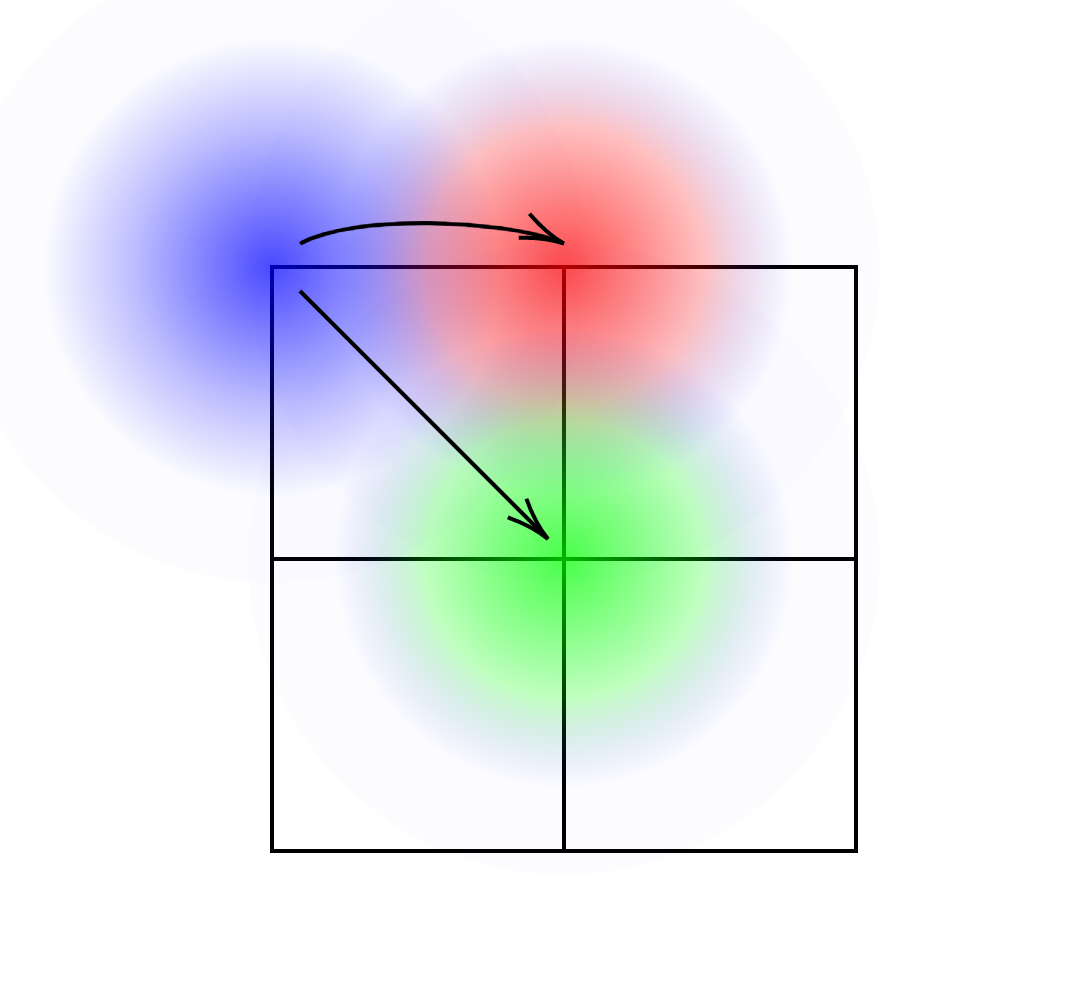
\includegraphics[width=0.4\textwidth]{band/hopping/overlap.png}
    }
    \subfigure[在我们使用Wannier波函数作为表象后,波函数本身的空间分布的细节消失,只留下“电子在哪个格点附近”的粗略信息;交叠较大的两个Wannier态之间容易发生跃迁(用较深的颜色表示),交叠较小的两个Wannier态之间的跃迁不容易发生(用较浅的颜色表示)]{
        

\tikzset{every picture/.style={line width=0.75pt}} %set default line width to 0.75pt        

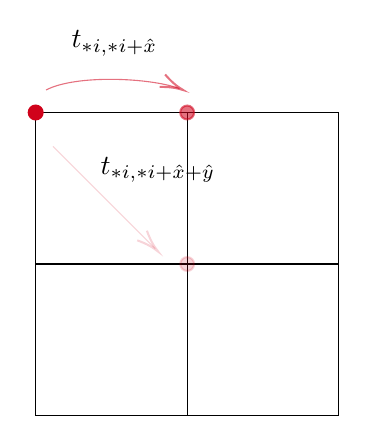
\begin{tikzpicture}[x=0.75pt,y=0.75pt,yscale=-1,xscale=1]
%uncomment if require: \path (0,300); %set diagram left start at 0, and has height of 300

%Shape: Grid [id:dp9196204391144727] 
\draw  [draw opacity=0] (186,104) -- (332,104) -- (332,250) -- (186,250) -- cycle ; \draw   (259,104) -- (259,250) ; \draw   (186,177) -- (332,177) ; \draw   (186,104) -- (332,104) -- (332,250) -- (186,250) -- cycle ;
%Straight Lines [id:da29204160455087] 
\draw [color={rgb, 255:red, 208; green, 2; blue, 27 }  ,draw opacity=0.56 ][fill={rgb, 255:red, 208; green, 2; blue, 27 }  ,fill opacity=0.13 ]   (259,104) ;
\draw [shift={(259,104)}, rotate = 0] [color={rgb, 255:red, 208; green, 2; blue, 27 }  ,draw opacity=0.56 ][fill={rgb, 255:red, 208; green, 2; blue, 27 }  ,fill opacity=0.56 ][line width=0.75]      (0, 0) circle [x radius= 3.35, y radius= 3.35]   ;
%Straight Lines [id:da29894868694295185] 
\draw [color={rgb, 255:red, 208; green, 2; blue, 27 }  ,draw opacity=0.17 ]   (194.33,120.33) -- (243.59,169.59) ;
\draw [shift={(245,171)}, rotate = 225] [color={rgb, 255:red, 208; green, 2; blue, 27 }  ,draw opacity=0.17 ][line width=0.75]    (10.93,-3.29) .. controls (6.95,-1.4) and (3.31,-0.3) .. (0,0) .. controls (3.31,0.3) and (6.95,1.4) .. (10.93,3.29)   ;
%Straight Lines [id:da865515748256444] 
\draw [color={rgb, 255:red, 208; green, 2; blue, 27 }  ,draw opacity=1 ][fill={rgb, 255:red, 208; green, 2; blue, 27 }  ,fill opacity=1 ]   (186,104) ;
\draw [shift={(186,104)}, rotate = 0] [color={rgb, 255:red, 208; green, 2; blue, 27 }  ,draw opacity=1 ][fill={rgb, 255:red, 208; green, 2; blue, 27 }  ,fill opacity=1 ][line width=0.75]      (0, 0) circle [x radius= 3.35, y radius= 3.35]   ;
%Straight Lines [id:da24429470745271376] 
\draw [color={rgb, 255:red, 208; green, 2; blue, 27 }  ,draw opacity=0.17 ][fill={rgb, 255:red, 208; green, 2; blue, 27 }  ,fill opacity=1 ]   (259,177) ;
\draw [shift={(259,177)}, rotate = 0] [color={rgb, 255:red, 208; green, 2; blue, 27 }  ,draw opacity=0.17 ][fill={rgb, 255:red, 208; green, 2; blue, 27 }  ,fill opacity=0.17 ][line width=0.75]      (0, 0) circle [x radius= 3.35, y radius= 3.35]   ;
%Curve Lines [id:da1801641720051903] 
\draw [color={rgb, 255:red, 208; green, 2; blue, 27 }  ,draw opacity=0.56 ]   (191,93.15) .. controls (205.4,85.65) and (241,87.19) .. (255.32,92.47) ;
\draw [shift={(257,93.15)}, rotate = 204.12] [color={rgb, 255:red, 208; green, 2; blue, 27 }  ,draw opacity=0.56 ][line width=0.75]    (10.93,-3.29) .. controls (6.95,-1.4) and (3.31,-0.3) .. (0,0) .. controls (3.31,0.3) and (6.95,1.4) .. (10.93,3.29)   ;

% Text Node
\draw (202,63.4) node [anchor=north west][inner sep=0.75pt]    {$t_{\vb*{i},\vb*{i}+\hat{x}}$};
% Text Node
\draw (216,124.4) node [anchor=north west][inner sep=0.75pt]    {$t_{\vb*{i},\vb*{i}+\hat{x} +\hat{y}}$};


\end{tikzpicture}

    }
    \subfigure[晶格中可以有不止一种原子(此图中有两种),每种原子周围可以不止一种轨道]{
        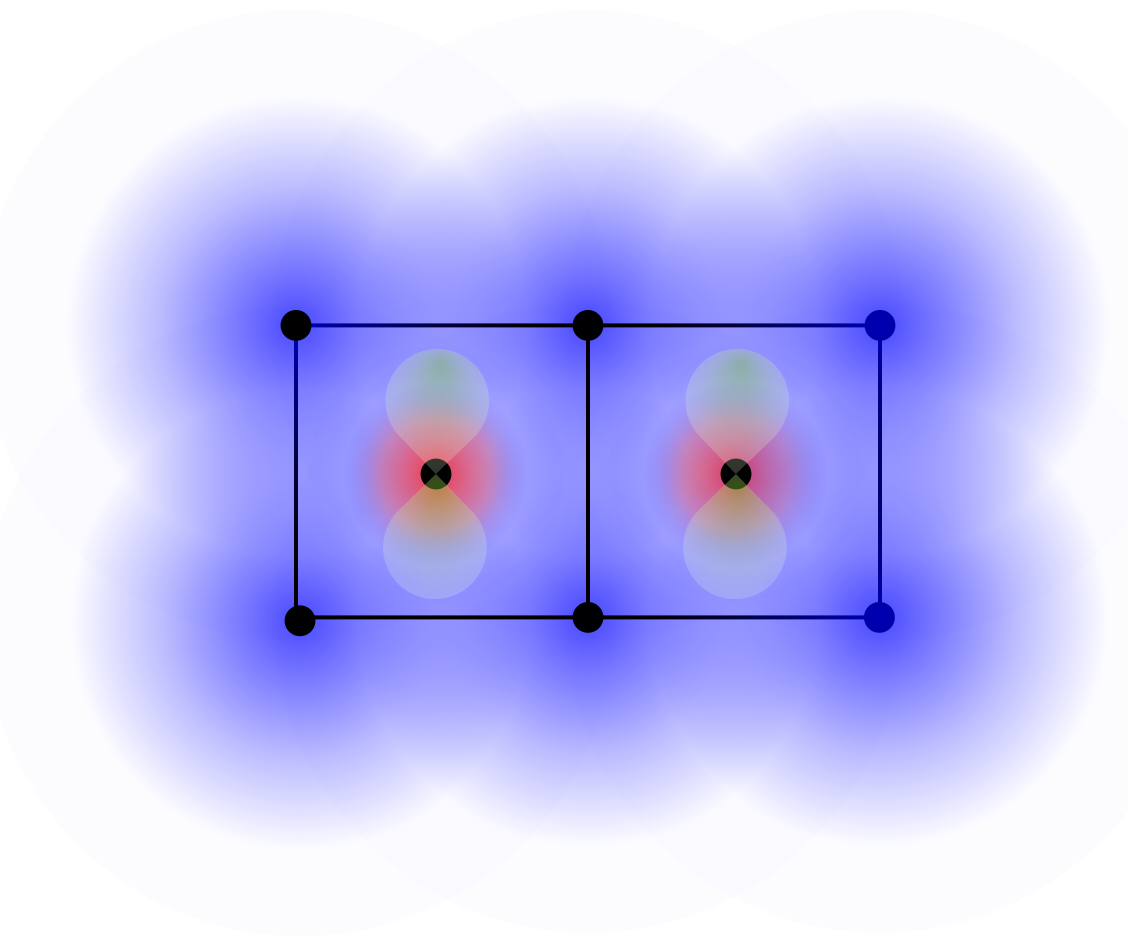
\includegraphics[width=0.5\textwidth]{band/hopping/lattice-multi-atoms.png}
    }
    \subfigure[最终的模型形如\eqref{eq:hamiltonian-in-wannier},其中的电子可以用两个标签标记,一个表示Wannier波函数,不同状态的电子之间的跃迁有强有弱,用颜色深浅表示]{
        

\tikzset{every picture/.style={line width=0.75pt}} %set default line width to 0.75pt        

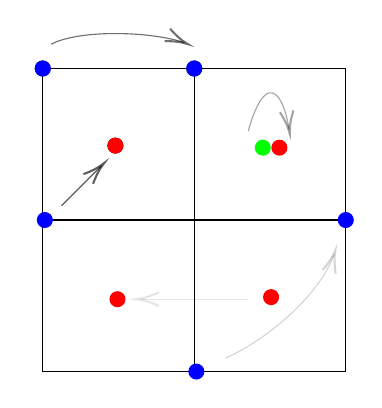
\begin{tikzpicture}[x=0.75pt,y=0.75pt,yscale=-1,xscale=1]
%uncomment if require: \path (0,300); %set diagram left start at 0, and has height of 300

%Shape: Grid [id:dp045220665097531976] 
\draw  [draw opacity=0] (207,161.85) -- (353,161.85) -- (353,234.85) -- (207,234.85) -- cycle ; \draw   (280,161.85) -- (280,234.85) ; \draw    ; \draw   (207,161.85) -- (353,161.85) -- (353,234.85) -- (207,234.85) -- cycle ;
%Shape: Grid [id:dp906158521242364] 
\draw  [draw opacity=0] (207,88.85) -- (353,88.85) -- (353,161.85) -- (207,161.85) -- cycle ; \draw   (280,88.85) -- (280,161.85) ; \draw    ; \draw   (207,88.85) -- (353,88.85) -- (353,161.85) -- (207,161.85) -- cycle ;
%Straight Lines [id:da08411653734161595] 
\draw [color={rgb, 255:red, 0; green, 0; blue, 0 }  ,draw opacity=1 ]   (242,126) ;
\draw [shift={(242,126)}, rotate = 0] [color={rgb, 255:red, 0; green, 0; blue, 0 }  ,draw opacity=1 ][fill={rgb, 255:red, 0; green, 0; blue, 0 }  ,fill opacity=1 ][line width=0.75]      (0, 0) circle [x radius= 3.35, y radius= 3.35]   ;
%Straight Lines [id:da6183208679206122] 
\draw [color={rgb, 255:red, 0; green, 0; blue, 0 }  ,draw opacity=1 ]   (280,88.85) ;
\draw [shift={(280,88.85)}, rotate = 0] [color={rgb, 255:red, 0; green, 0; blue, 0 }  ,draw opacity=1 ][fill={rgb, 255:red, 0; green, 0; blue, 0 }  ,fill opacity=1 ][line width=0.75]      (0, 0) circle [x radius= 3.35, y radius= 3.35]   ;
%Straight Lines [id:da8539422417305953] 
\draw [color={rgb, 255:red, 0; green, 0; blue, 0 }  ,draw opacity=1 ]   (207,88.85) ;
\draw [shift={(207,88.85)}, rotate = 0] [color={rgb, 255:red, 0; green, 0; blue, 0 }  ,draw opacity=1 ][fill={rgb, 255:red, 0; green, 0; blue, 0 }  ,fill opacity=1 ][line width=0.75]      (0, 0) circle [x radius= 3.35, y radius= 3.35]   ;
%Straight Lines [id:da8210604270560764] 
\draw [color={rgb, 255:red, 0; green, 0; blue, 255 }  ,draw opacity=1 ]   (207,88.85) ;
\draw [shift={(207,88.85)}, rotate = 0] [color={rgb, 255:red, 0; green, 0; blue, 255 }  ,draw opacity=1 ][fill={rgb, 255:red, 0; green, 0; blue, 255 }  ,fill opacity=1 ][line width=0.75]      (0, 0) circle [x radius= 3.35, y radius= 3.35]   ;
%Straight Lines [id:da7554787979553312] 
\draw [color={rgb, 255:red, 255; green, 0; blue, 0 }  ,draw opacity=1 ]   (242,126) ;
\draw [shift={(242,126)}, rotate = 0] [color={rgb, 255:red, 255; green, 0; blue, 0 }  ,draw opacity=1 ][fill={rgb, 255:red, 255; green, 0; blue, 0 }  ,fill opacity=1 ][line width=0.75]      (0, 0) circle [x radius= 3.35, y radius= 3.35]   ;
%Straight Lines [id:da24259314385484876] 
\draw [color={rgb, 255:red, 0; green, 0; blue, 255 }  ,draw opacity=1 ]   (280,88.85) ;
\draw [shift={(280,88.85)}, rotate = 0] [color={rgb, 255:red, 0; green, 0; blue, 255 }  ,draw opacity=1 ][fill={rgb, 255:red, 0; green, 0; blue, 255 }  ,fill opacity=1 ][line width=0.75]      (0, 0) circle [x radius= 3.35, y radius= 3.35]   ;
%Curve Lines [id:da07826906250230103] 
\draw [color={rgb, 255:red, 0; green, 0; blue, 0 }  ,draw opacity=0.57 ]   (211,77.15) .. controls (225.4,69.65) and (261,71.19) .. (275.32,76.47) ;
\draw [shift={(277,77.15)}, rotate = 204.12] [color={rgb, 255:red, 0; green, 0; blue, 0 }  ,draw opacity=0.57 ][line width=0.75]    (10.93,-3.29) .. controls (6.95,-1.4) and (3.31,-0.3) .. (0,0) .. controls (3.31,0.3) and (6.95,1.4) .. (10.93,3.29)   ;
%Straight Lines [id:da6887699530150242] 
\draw [color={rgb, 255:red, 255; green, 0; blue, 0 }  ,draw opacity=1 ]   (321,127) ;
\draw [shift={(321,127)}, rotate = 0] [color={rgb, 255:red, 255; green, 0; blue, 0 }  ,draw opacity=1 ][fill={rgb, 255:red, 255; green, 0; blue, 0 }  ,fill opacity=1 ][line width=0.75]      (0, 0) circle [x radius= 3.35, y radius= 3.35]   ;
%Straight Lines [id:da8877871041262482] 
\draw    (200,224) ;
%Straight Lines [id:da7839745415328059] 
\draw [color={rgb, 255:red, 0; green, 255; blue, 0 }  ,draw opacity=1 ]   (313,127) ;
\draw [shift={(313,127)}, rotate = 0] [color={rgb, 255:red, 0; green, 255; blue, 0 }  ,draw opacity=1 ][fill={rgb, 255:red, 0; green, 255; blue, 0 }  ,fill opacity=1 ][line width=0.75]      (0, 0) circle [x radius= 3.35, y radius= 3.35]   ;
%Curve Lines [id:da4448019114782187] 
\draw [color={rgb, 255:red, 0; green, 0; blue, 0 }  ,draw opacity=0.36 ]   (306,119) .. controls (313.76,91.19) and (322.46,97.89) .. (325.71,118.39) ;
\draw [shift={(326,120.33)}, rotate = 262.23] [color={rgb, 255:red, 0; green, 0; blue, 0 }  ,draw opacity=0.36 ][line width=0.75]    (10.93,-3.29) .. controls (6.95,-1.4) and (3.31,-0.3) .. (0,0) .. controls (3.31,0.3) and (6.95,1.4) .. (10.93,3.29)   ;
%Straight Lines [id:da8222874180206843] 
\draw [color={rgb, 255:red, 0; green, 0; blue, 255 }  ,draw opacity=1 ]   (208,161.85) ;
\draw [shift={(208,161.85)}, rotate = 0] [color={rgb, 255:red, 0; green, 0; blue, 255 }  ,draw opacity=1 ][fill={rgb, 255:red, 0; green, 0; blue, 255 }  ,fill opacity=1 ][line width=0.75]      (0, 0) circle [x radius= 3.35, y radius= 3.35]   ;
%Straight Lines [id:da12806615593183923] 
\draw [color={rgb, 255:red, 0; green, 0; blue, 0 }  ,draw opacity=0.63 ]   (216,155) -- (235.25,135.75) ;
\draw [shift={(236.67,134.33)}, rotate = 495] [color={rgb, 255:red, 0; green, 0; blue, 0 }  ,draw opacity=0.63 ][line width=0.75]    (10.93,-3.29) .. controls (6.95,-1.4) and (3.31,-0.3) .. (0,0) .. controls (3.31,0.3) and (6.95,1.4) .. (10.93,3.29)   ;
%Straight Lines [id:da48135278956803007] 
\draw [color={rgb, 255:red, 0; green, 0; blue, 255 }  ,draw opacity=1 ]   (353,161.85) ;
\draw [shift={(353,161.85)}, rotate = 0] [color={rgb, 255:red, 0; green, 0; blue, 255 }  ,draw opacity=1 ][fill={rgb, 255:red, 0; green, 0; blue, 255 }  ,fill opacity=1 ][line width=0.75]      (0, 0) circle [x radius= 3.35, y radius= 3.35]   ;
%Straight Lines [id:da1581276506967122] 
\draw [color={rgb, 255:red, 0; green, 0; blue, 255 }  ,draw opacity=1 ]   (281,234.85) ;
\draw [shift={(281,234.85)}, rotate = 0] [color={rgb, 255:red, 0; green, 0; blue, 255 }  ,draw opacity=1 ][fill={rgb, 255:red, 0; green, 0; blue, 255 }  ,fill opacity=1 ][line width=0.75]      (0, 0) circle [x radius= 3.35, y radius= 3.35]   ;
%Curve Lines [id:da9474868662390499] 
\draw [color={rgb, 255:red, 0; green, 0; blue, 0 }  ,draw opacity=0.17 ]   (295,228.33) .. controls (313.43,220.57) and (340.33,198.7) .. (347.4,178.23) ;
\draw [shift={(348,176.33)}, rotate = 465.95] [color={rgb, 255:red, 0; green, 0; blue, 0 }  ,draw opacity=0.17 ][line width=0.75]    (10.93,-3.29) .. controls (6.95,-1.4) and (3.31,-0.3) .. (0,0) .. controls (3.31,0.3) and (6.95,1.4) .. (10.93,3.29)   ;
%Straight Lines [id:da23223153967612653] 
\draw [color={rgb, 255:red, 255; green, 0; blue, 0 }  ,draw opacity=1 ]   (317,199) ;
\draw [shift={(317,199)}, rotate = 0] [color={rgb, 255:red, 255; green, 0; blue, 0 }  ,draw opacity=1 ][fill={rgb, 255:red, 255; green, 0; blue, 0 }  ,fill opacity=1 ][line width=0.75]      (0, 0) circle [x radius= 3.35, y radius= 3.35]   ;
%Straight Lines [id:da3389787384317531] 
\draw [color={rgb, 255:red, 255; green, 0; blue, 0 }  ,draw opacity=1 ]   (243,200) ;
\draw [shift={(243,200)}, rotate = 0] [color={rgb, 255:red, 255; green, 0; blue, 0 }  ,draw opacity=1 ][fill={rgb, 255:red, 255; green, 0; blue, 0 }  ,fill opacity=1 ][line width=0.75]      (0, 0) circle [x radius= 3.35, y radius= 3.35]   ;
%Straight Lines [id:da5291303318619174] 
\draw [color={rgb, 255:red, 0; green, 0; blue, 0 }  ,draw opacity=0.1 ]   (306,200) -- (254,200) ;
\draw [shift={(252,200)}, rotate = 360] [color={rgb, 255:red, 0; green, 0; blue, 0 }  ,draw opacity=0.1 ][line width=0.75]    (10.93,-3.29) .. controls (6.95,-1.4) and (3.31,-0.3) .. (0,0) .. controls (3.31,0.3) and (6.95,1.4) .. (10.93,3.29)   ;




\end{tikzpicture}

    }
    \caption{\eqref{eq:hamiltonian-in-wannier}的直观展示}
\end{figure}

\subsubsection{简单晶格的原子轨道线性组合(LCAO)} 

在简单晶格中,如果不同原子的轨道基本上没有重叠,那实际上单原子轨道波函数就是Wannier波函数。
设不同原子的轨道没有什么重叠,则有
\begin{equation}
    \int \dd[3]{\vb*{r}} \varphi_n^*(\vb*{r} - \vb*{R}_i) \varphi_n(\vb*{r} - \vb*{R}_j) = \delta_{ij},
    \label{eq:no-overlap-atom-orbital}
\end{equation}
$i=j$时上式显然是$1$,$i \neq j$时由于两个波函数没有重叠,就是零,因此上式的确是成立的。
$\varphi_n(\vb*{r} - \vb*{R}_i)$满足
\begin{equation}
    \left( - \frac{\laplacian}{2m} + V_\text{atom} (\vb*{r} - \vb*{R}_i) \right) \varphi_n(\vb*{r} - \vb*{R}_i) = \epsilon_n \varphi_n(\vb*{r} - \vb*{R}_i),
\end{equation}
而能带电子的波函数满足
\begin{equation}
    \left( - \frac{\laplacian}{2m} + V (\vb*{r}) \right) \psi_{n \vb*{k}} = \epsilon_{n \vb*{k}} \psi_{n \vb*{k}},
\end{equation}
我们现在做展开
\begin{equation}
    \psi_{n \vb*{k}}(\vb*{r}) = \sum_i a_i \varphi_n(\vb*{r} - \vb*{R}_i),
\end{equation}
就得到
\[
    \sum_i a_i (\epsilon_n + V(\vb*{r}) - V_\text{atom}(\vb*{r} - \vb*{R}_i)) \varphi_n(\vb*{r} - \vb*{R}_i) = \epsilon_{n \vb*{k}} \sum_i a_i \varphi_i(\vb*{r} - \vb*{R}_i),
\]
两边作用\eqref{eq:no-overlap-atom-orbital},就得到
\begin{equation}
    (\epsilon_{n \vb*{k}} - \epsilon_n) a_i = \sum_{j} a_j \int \dd[3]{\vb*{r}} \varphi_n(\vb*{r} - \vb*{R}_i)^* ( V(\vb*{r}) - V_\text{atom}(\vb*{r} - \vb*{R}_i)) \varphi_n(\vb*{r} - \vb*{R}_j).
\end{equation}

总之,在原子轨道波函数之间真的没有什么交叠的情况下,原子轨道波函数就是Wannier波函数。
然而,在大多数情况下,原子轨道波函数还是比较不局域的,我们需要先从原子轨道波函数出发计算得到Bloch波函数,然后做傅里叶变换得到比原子轨道波函数更加局域的Wannier波函数。

如果只有最近邻或是次近邻的跃迁,那么我们就有一个非常直观的物理图像:似乎可以用“某个电子正在某个格点附近”来标记一个电子,即电子似乎被紧紧地束缚在晶格上,无法长距离移动,这就是“紧束缚”一词的来历。
或者,也有可能电子并不是特别局域,但是原子间距很大,以至于在系统中电子通常具有的动能下,非常远距离的跃迁似乎无法一次完成。
这就是说,紧束缚模型中,电子的动能不应该能够到达特别大,从而也不应该有太大的能带带宽(的确应该考虑带宽而不是能量的绝对大小,因为总是可以通过化学势来任意增减能量,而上面的物理图像和化学势毫无关系)。
还可以从另一个角度看这个现象:我们知道自由电子的动能项在动量表象下是对角化的,这意味着它在坐标表象下是非常不对角化的,体现在$i$表象中就是有非常远的跃迁。
另一方面,晶格势能项在坐标表象下是对角化的,体现在$i$表象中就是$\epsilon_i c^\dagger_i c_i$型的项占据压倒性优势。
因此,单电子越是被束缚,其哈密顿量就越像晶格势能项,只涉及很近邻的跃迁,而越是自由,其哈密顿量就越像自由电子的哈密顿量,涉及很远的跃迁。

\subsubsection{复式晶格的LCAO} 

可以先假装轨道波函数真的是Wannier波函数,然后做杂化


\subsection{坐标表象作为一种Wannier表象} 

如果用以自行设定的用不同电子轨道线性组合得到的Wannier波函数为表象,这个表象下的波函数只能够展示电子在不同晶胞上的概率振幅分布,保留了一些“一个电子是哪些轨道的混合”的信息,能带编号比较清晰。
以自行设定的用不同电子轨道线性组合得到的Bloch波函数为表象。波函数不显示任何电子的空间分布信息,但是保留了一些“一个电子是哪些轨道的混合”的信息。

\subsection{表象变换总结} 

总结一下,形如\eqref{eq:hamiltonian-in-wannier}的近独立电子模型最大的好处在于提供了介于哈密顿量完全对角化的Bloch波函数表象(或者说晶格动量表象)和完全没有做过任何处理的坐标表象之间的许多表象。
我们上面提到过的表象从坐标表象到晶格动量表象形成如下序列:
\begin{enumerate}
    \item \eqref{eq:electron-gas-hamiltonian},完全就是“自由电子气动能加势能”,没有做任何处理。最容易写下哈密顿量,最难以理解其物理。这种表象下的波函数清楚地展示了电子在空间各点的概率振幅分布,但是没有提供关于$\vb*{k}$和$n$的任何信息。
    \item 以单原子轨道为表象。相对容易写下来哈密顿量。这种表象下的波函数无法展示每个轨道具体长什么样的信息(因为轨道编号只是一个抽象的量子数),但电子出现在不同原子附近的概率振幅的信息保留了。第一次出现了和能带编号有关的标签(轨道编号)。
    \item 以单原子内部的杂化轨道为表象。电子出现在不同原子附近的概率振幅的信息保留了。杂化轨道的编号是能带编号的更好的近似,即能带编号开始清晰起来。
    \item 以原子间的成键和反键轨道为表象。电子出现在不同原子附近的概率振幅的信息被模糊化了,但是能带编号变得更清晰了。
    \item \eqref{eq:multi-band-tight-binding},离完全对角化的$\epsilon = \epsilon_{\vb*{k}}$只有一步之遥。这个表象下的波函数只能够展示电子在不同晶胞上的概率振幅分布,能带编号非常清晰,而原来的单原子轨道完全模糊了。
    \item 能带$\epsilon = \epsilon_{n\vb*{k}}$。波函数不展示任何电子的空间分布信息,也没有任何关于单原子轨道的信息,只有确定的晶格动量和能带编号。
\end{enumerate}

从上到下,坐标变得模糊而动量变得清晰:先是单原子波函数的细节模糊了,然后是电子在晶格内的哪个原子附近(或者说,复式晶格中在哪套子格子附近)变得模糊了,最后电子在哪个晶胞附近也模糊了,而$\vb*{k}$变得清晰了。
单电子轨道标签先是出现(作为单原子波函数的细节模糊的补偿),然后变得模糊了:先是杂化,然后是成键、反键,单原子轨道的信息逐步丢失,而越来越像正确的能带标签。
凝聚态理论研究中通常不会采取这个序列两端的表象,因为它们过于复杂而难以做近似。
这就是紧束缚模型的重要之处,虽然当代已经没人用它做任何第一性原理计算了。

% TODO:两种k是一样的
在\eqref{eq:hamiltonian-in-wannier}的对角化,即讨论它和Bloch表象下的能带之间的关系。
将电子的产生湮灭算符$c_{mi}^\dagger$做傅里叶变换\eqref{eq:lattice-fourier},将\eqref{eq:hamiltonian-in-wannier}写成对角化的,立刻可以看出有能带产生。因此Wannier电子经过一个线性变换,也会变成能带电子。
根据\autoref{sec:momentum-space-inner-product}中的论证,\eqref{eq:hamiltonian-in-wannier}不会有$1/N$或是$1/V$之类的因子出现。
因此实际上\eqref{eq:lattice-fourier}给出的$\vb*{k}$表象和从自由电子出发得到的限制在第一布里渊区中的简约波矢标记的Bloch电子是同样的表象,因为两者对角化完成后均形如。

\section{电磁场耦合}

电磁场

\section{相互作用通道}

\subsection{相互作用通道}\label{sec:interaction-bloch}

本节讨论从自由电子模型出发如何加入相互作用。对库伦相互作用,有
\[
    \begin{aligned}
        H_{\vb*{k}_4 \vb*{k}_3 \vb*{k}_2 \vb*{k}_1} &= \frac{1}{2} \int \dd[3]{\vb*{r}} \int \dd[3]{\vb*{r}'} \braket*{\vb*{k}_4}{\vb*{r}} \braket*{\vb*{k}_3}{\vb*{r}'} V(\vb*{r} - \vb*{r}') \braket*{\vb*{r}'}{\vb*{k}_2} \braket*{\vb*{r}}{\vb*{k}_1}  \\
        &= \frac{1}{2 V^2} \int \dd[3]{\vb*{r}} \int \dd[3]{\vb*{r}'} \ee^{\ii (\vb*{k}_2 - \vb*{k}_3) \cdot \vb*{r}'} \ee^{\ii (\vb*{k}_1 - \vb*{k}_4) \cdot \vb*{r}} V(\vb*{r} - \vb*{r}') \\
        &= \frac{1}{2V^2} \int \dd[3]{\vb*{r}} \int \dd[3]{\vb*{r}'} \ee^{- \ii (\vb*{k}_3 + \vb*{k}_4 - \vb*{k}_1 - \vb*{k}_2) \cdot \vb*{r}'} \ee^{- \ii(\vb*{k}_2 - \vb*{k}_3) \cdot \vb*{r}} V(\vb*{r}) \\
        &= \frac{1}{2V} \delta_{\vb*{k}_3 + \vb*{k}_4, \vb*{k}_1 + \vb*{k}_2} \int \dd[3]{\vb*{r}} \ee^{- \ii (\vb*{k}_2 - \vb*{k}_3) \cdot \vb*{r}} V(\vb*{r}),
    \end{aligned}
\]
我们定义
\[
    \vb*{q} = \vb*{k}_2 - \vb*{k}_3,
\]
就得到
\begin{equation}
    H_{\vb*{k}_1 + \vb*{q}, \vb*{k}_2 - \vb*{q}, \vb*{k}_2, \vb*{k}_1} = \frac{1}{2V} \int \dd[3]{\vb*{r}} \ee^{- \ii \vb*{q} \cdot \vb*{r}} V(\vb*{r}),
\end{equation}
或者说
\begin{equation}
    H_\text{int} = \frac{1}{2V} \sum_{\vb*{k}_1, \vb*{k}_2, \vb*{q}} V_{\vb*{q}} c^\dagger_{\vb*{k}_1 + \vb*{q}} c^\dagger_{\vb*{k}_2 - \vb*{q}} c_{\vb*{k}_2} c_{\vb*{k}_1} , \quad V_{\vb*{q}} = \int \dd[3]{\vb*{r}} \ee^{- \ii \vb*{q} \cdot \vb*{r}} V(\vb*{r}).
\end{equation}
如果考虑自旋,就有
\begin{equation}
    H_\text{int} = \frac{1}{2V} \sum_{\alpha, \beta} \sum_{\vb*{k}_1, \vb*{k}_2, \vb*{q}} V_{\vb*{q}} c^\dagger_{\vb*{k}_1 + \vb*{q}, \alpha} c^\dagger_{\vb*{k}_2 - \vb*{q}, \beta} c_{\vb*{k}_2 \beta} c_{\vb*{k}_1 \alpha}.
\end{equation}

\subsection{单能带系统的相互作用哈密顿量}

对单带模型,在Wannier表象下,库仑相互作用可以表示成如下矩阵元形式:
\begin{equation}
    \begin{aligned}
        H_{i i' j' j} &= \frac{1}{2} \int \dd[3]{\vb*{r}} \int \dd[3]{\vb*{r}'} \braket{i}{\vb*{r}} \braket{i'}{\vb*{r}'} V(\vb*{r} - \vb*{r}') \braket{\vb*{r}'}{j'} \braket{\vb*{r}}{j} \\
        &= \frac{1}{2} \int \dd[3]{\vb*{r}} \int \dd[3]{\vb*{r}'} w_i^*(\vb*{r}) w_{i'}^*(\vb*{r}') V(\vb*{r} - \vb*{r}') w_{j'}(\vb*{r}') w_j(\vb*{r}),
    \end{aligned}
    \label{eq:wannier-basis-interaction}
\end{equation}
于是总的哈密顿量为
\begin{equation}
    H = \sum_{i, i', \sigma} c^\dagger_{i \sigma} t_{i i'} c_{i' \sigma} + \sum_{i, i', j, j', \sigma, \sigma'} V_{i i' j' j} c^\dagger_{i \sigma} c^\dagger_{i' \sigma'} c_{j' \sigma'} c_{j \sigma}.
\end{equation}

对上式做傅里叶变换,使用\eqref{eq:lattice-fourier}会有$1/2N$的因子,然而\autoref{sec:momentum-space-inner-product}也论证了,从$\vb*{r}$表象切换到动量表象后,二体相互作用项会有$1/2V$的因子。
\autoref{sec:tight-binding-hopping}中已经论证了,无论是自由电子气模型加入周期势扰动,然后做傅里叶变换得到的$\vb*{k}$表象和对上式做傅里叶变换得到的$\vb*{k}$表象就是一个东西,所以看起来似乎有矛盾。
实际上两者没有矛盾,因为\autoref{sec:momentum-space-inner-product}中的二体相互作用的耦合常数直接就是$V_{\vb*{q}}$,但是本节中的二体相互作用的耦合常数是$V_{i i' j j'}$傅里叶变换而来,根据\eqref{eq:wannier-and-free},两者的确应该差一个$V_\text{u.c.}$因子。

与自由电子气模型或凝胶模型不同,紧束缚模型对相互作用是非常敏感的,不能保证加入(即使比较弱的)相互作用后,系统能够用费米液体理论(见\autoref{sec:landau-fermi-liquid})描述,甚至不能保证能带仍然是具有明确物理意义的。
这是出于一个非常直观的原因:紧束缚模型的能带通常更窄,从而态密度更大,从而库伦散射更明显,从而也更加容易在相互作用加入之后变成强关联系统。
或者,我们也可以如此理解紧束缚模型对相互作用的敏感性:由于电子动能不能取特别大的值,相比之下相互作用能量应该占据主导,从而系统具有强关联效应。

总之,以下几个说法基本上是等价的:
\begin{enumerate}
    \item 系统可以用紧束缚模型或者考虑了次近邻、再次近邻的紧束缚模型加上一个相互作用项描述;
    \item 系统中的电子跃迁能力不大;
    \item 系统能带不宽;
    \item 系统中电子动能有较低的上限。
\end{enumerate}
满足这些条件的模型通常对相互作用更加敏感,也更加容易出现强关联效应。
这就导致了一个非常有趣的现象:一些数值计算方法,如DMRG,需要将所有自由度都定义在晶格上,从而,它们可以毫无困难地用于模拟很大一类强关联系统,但是却无法用于有效地模拟普通的费米液体系统。

需要注意,并非所有强关联系统都出现在紧束缚模型中。费米液体系统加入了适当的相互作用之后也可以出现强关联效应,此时使用基于格点的计算方法就不能获得很好的效果了。

\subsection{紧束缚近似成立时的单带相互作用通道}\label{sec:single-band-interaction-channel}

原则上$U_{i i' j' j}$对很多不同的$i, i', j', j$组合都有非零值。物理上这是很好理解的,因为库伦相互作用可以将任意原子附近的两个电子散射到任意的其它地方,由于高度定域的电子动量不确定,这里无所谓动量守恒的约束。
然而,在紧束缚模型成立时,足够大的矩阵元的$i, i', j', j$中,$j$和$j'$不是最近邻,就是完全一样(即所谓on-site repulsion)。
由于Wannier波函数高度定域,从\eqref{eq:wannier-basis-interaction}中可以看出,仅有的可能是$i=i'=j=j'$,或是$i=j \neq i'=j'$,或是$i=j' \neq i' = j$。
于是就有
\[
    \begin{aligned}
        &\quad \sum_{i, i', j, j', \sigma, \sigma'} V_{i i' j' j} c^\dagger_{i \sigma} c^\dagger_{i' \sigma'} c_{j' \sigma'} c_{j \sigma} \\
        &= \sum_{i, \sigma, \sigma'} V_{iiii} c^\dagger_{i \sigma} c^\dagger_{i \sigma'} c_{i \sigma'} c_{i \sigma} 
        + \sum_{i, j, \sigma, \sigma'} V_{i j j i} c^\dagger_{i \sigma} c^\dagger_{j \sigma'} c_{j \sigma'} c_{i \sigma}
        + \sum_{i, j, \sigma, \sigma'} V_{i j i j} c^\dagger_{i \sigma} c^\dagger_{j \sigma'} c_{i \sigma'} c_{j \sigma},
    \end{aligned}
\]
第一项为
\[
    \begin{aligned}
        \sum_{i, \sigma, \sigma'} V_{iiii} c^\dagger_{i \sigma} c^\dagger_{i \sigma'} c_{i \sigma'} c_{i \sigma} &= 2 \sum_{i} V_{iiii} n_{i \uparrow} n_{i \downarrow} + \sum_{i} U_{iiii} n_i \\
        &= \sum_{i} U_i n_{i \uparrow} n_{i \downarrow} + \frac{1}{2} \sum_{i} U_{i} n_i,
    \end{aligned}
\]
这里我们重新定义
\begin{equation}
    U_i = 2 V_{iiii}.
\end{equation}
第二项实际上是密度-密度相互作用,即为
\[
    \sum_{i, j, \sigma, \sigma'} V_{i j j i} c^\dagger_{i \sigma} c^\dagger_{j \sigma'} c_{j \sigma'} c_{i \sigma} = \sum_{\pair{i, j}} V_{ij} n_i n_j,
\]
其中我们重新定义了$V_{ij} = V_{ijji}$。使用公式
\[
    \vb*{\sigma}_{\alpha \beta} \cdot \vb*{\sigma}_{\alpha' \beta'} = 2 \delta_{\alpha \beta'} \delta_{\beta \alpha'} - \delta_{\alpha \beta} \delta_{\alpha' \beta'},
\]
可以验证
\[
    \sum_{i, j, \sigma, \sigma'} V_{i j i j} c^\dagger_{i \sigma} c^\dagger_{j \sigma'} c_{i \sigma'} c_{j \sigma} = - 2 \sum_{\pair{i, j}} V_{i j i j} \left( \vb*{S}_{i} \cdot \vb*{S}_j + \frac{1}{4} n_i n_j \right).
\]
我们把上式右边的第二项吸收进$V_{ij}$中,并且重新定义$2V_{ijij}=J_{ij}$,于是总的相互作用哈密顿量就是
\[
    \sum_{i} U_i n_{i \uparrow} n_{i \downarrow} + \sum_{\pair{i, j}} V_{ij} n_i n_j - \sum_{\pair{i, j}} J_{i j} \vb*{S}_{i} \cdot \vb*{S}_j + \sum_{i} U_i n_i.
\]
由空间平移对称性,on-site repulsion肯定是均一的,这样我们可以将$\sum_i U_i n_i$丢进化学势中;而如果它不是均一的,就意味着系统实际上不具有完美的离散平移对称结构,即系统中存在无序,直观地看,就是散布的杂质对电子产生散射,这基本上是一个单体算符,于是我们就得到了紧束缚模型最一般的哈密顿量:
\begin{equation}
    H = - \sum_{\pair{i, j}, \sigma} t_{ij} c^\dagger_{i \sigma} c_{j \sigma} 
    + \sum_{i} U_i n_{i \uparrow} n_{i \downarrow} 
    + \sum_{\pair{i, j}} V_{ij} n_i n_j - \sum_{\pair{i, j}} J_{i j} \vb*{S}_{i} \cdot \vb*{S}_j 
    - \mu \sum_i n_i + \sum_{i, j, \sigma, \sigma'} \epsilon_{ij\alpha \beta} c^\dagger_{i \alpha} c_{j \beta}.  
\end{equation}
这里的每一项都是有意义的,从左到右分别是:
\begin{enumerate}
    \item 动能项,衡量电子在格点之间跳跃的可能性;
    \item on-site repulsion,仅考虑这个相互作用得到的模型是所谓\concept{Hubbard模型};
    \item 密度-密度相互作用项,可能导致系统中出现持续的、不能平息的电子密度涨落,即所谓电荷密度波;
    \item 自旋-自旋相互作用项,可能导致出现自旋密度波,这一项意味着在有多个轨道的情况下,每个轨道上放置一个电子,且所有电子的自旋都平行时,系统能量最低,这是洪特规则的一个例子,不过通常说的“洪特相互作用”很多时候指的同个原子的各个壳层电子之间的相互作用;
    \item 化学势,调节系统中电子个数;
    \item 无序,可能来自杂质或是晶格的缺陷。
\end{enumerate}

\subsection{紧束缚近似成立时的多能带相互作用通道}

以上的讨论集中在单能带模型中。在有多个能带时,我们需要使用八个标签标记相互作用通道:有四个标签标记格点,四个标签标记能带编号。
对格点的标签,可以使用\autoref{sec:single-band-interaction-channel}开头的论证,仅有的可能是$i=i'=j=j'$,或是$i=j \neq i'=j'$,或是$i=j' \neq i' = j$,所以我们只需要讨论不同能带之间的相互作用情况。

对on-site repulsion项,即$i=i'=j=j'$的情况,容易看出其多能带版本是
\[
    \sum_{i, \sigma, \sigma'} \sum_{m, m', n, n'} V_{iiii,mm' nn'} c^\dagger_{i m \sigma} 
\]

实际的原子内部的洪特规则应该就是在这里能够拿到

\subsection{能带理论何时失效?}

基本自由度\emph{不能}写成经过相互作用修饰的能带电子的系统通常称为\concept{强关联系统},因为电子和电子之间的关系是如此剧烈,以至于单电子图像根本就是不可靠的。
本节给出一些能够暗示能带理论失效的判据,并且列举强关联系统通常会有什么性质。

如果能带计算出现平带,即非常窄的能带,则容易出现强关联系统。
可以从好几个角度看这个现象:态密度反比于群速度,从而能带越窄,态密度越大,自然相互作用也越大;能带窄也意味着电子动能低,因此相互作用能不需要太大就能够产生显著的效果。
如前所述,紧束缚模型通常具有这种特征,向紧束缚模型加入相互作用是容易产生强关联系统的。

即使是能带理论失效的情况下,能带的概念也是有意义的,因为它毕竟提供了一个合理的“自由理论”,我们可以向它加入各种相互作用来得到合适的强关联理论。